\documentclass[10pt,aspectratio=169]{beamer}

\usepackage[utf8]{inputenc}
\usepackage[utf8]{vietnam}
\usepackage{lmodern}
\usepackage{booktabs}
\usepackage{colortbl}
\usepackage{graphicx}
\usepackage{tikz}
\usepackage{array}
\usepackage{amsmath}
\usepackage{hyperref}
\usetikzlibrary{positioning}

\usetheme{default}
\usefonttheme{professionalfonts}
\renewcommand{\familydefault}{\sfdefault}

% ---------- Bảng màu HCMUS ----------
\definecolor{HCMUSBlue}{HTML}{123B67}
\definecolor{HCMUSTeal}{HTML}{008C95}
\definecolor{HCMUSLight}{HTML}{EAF3F5}
\definecolor{HCMUSRed}{HTML}{D94B4B}
\definecolor{HCMUSGreen}{HTML}{2E8B57}
\definecolor{TextDark}{HTML}{243447}
\definecolor{MutedText}{HTML}{5F6B76}
\definecolor{SoftGray}{HTML}{F4F6F8}

\setbeamercolor{normal text}{fg=TextDark,bg=white}
\setbeamercolor{structure}{fg=HCMUSBlue}
\setbeamercolor{frametitle}{fg=white,bg=HCMUSBlue}
\setbeamercolor{title}{fg=white}
\setbeamercolor{subtitle}{fg=HCMUSLight}
\setbeamercolor{author}{fg=white}
\setbeamercolor{date}{fg=HCMUSLight}
\setbeamercolor{block title}{fg=white,bg=HCMUSBlue}
\setbeamercolor{block body}{fg=TextDark,bg=HCMUSLight}
\setbeamercolor{alerted text}{fg=HCMUSRed}

\setbeamertemplate{navigation symbols}{}
\setbeamertemplate{items}[circle]
\setbeamersize{text margin left=0.65cm,text margin right=0.65cm}

\setbeamertemplate{frametitle}{%
  \nointerlineskip
  \begin{beamercolorbox}[wd=\paperwidth,ht=0.78cm,dp=0.20cm,leftskip=0.65cm]{frametitle}
    \usebeamerfont{frametitle}\insertframetitle
  \end{beamercolorbox}
}

\setbeamertemplate{footline}{%
  \leavevmode
  \begin{beamercolorbox}[wd=\paperwidth,ht=0.30cm,dp=0.13cm,leftskip=0.65cm,rightskip=0.65cm]{normal text}
    \color{MutedText}\scriptsize
    Mô hình hoá thống kê \hfill
    Phân tích Employee Attrition \hfill
    \insertframenumber/\inserttotalframenumber
  \end{beamercolorbox}
}

\setbeamertemplate{title page}{%
  \begin{tikzpicture}[remember picture,overlay]
    \fill[HCMUSBlue] (current page.south west) rectangle (current page.north east);
    \fill[HCMUSTeal] (current page.south west)
      rectangle ([xshift=0.18cm]current page.north west);
    \fill[HCMUSTeal,opacity=0.18]
      ([xshift=-4.0cm,yshift=-1.0cm]current page.north east) circle (2.8cm);
    \fill[white,opacity=0.06]
      ([xshift=-1.0cm,yshift=0.2cm]current page.south east) circle (3.2cm);
  \end{tikzpicture}
  \vspace{0.15cm}
  \begin{columns}[T,onlytextwidth]
    \begin{column}{0.76\textwidth}
      {\usebeamerfont{title}\color{white}\LARGE\bfseries
       Phân tích các yếu tố liên hệ với\\[0.08cm]
       quyết định nghỉ việc\par}
      \vspace{0.28cm}
      {\color{HCMUSLight}\large IBM HR Employee Attrition}
      \vspace{0.65cm}

      {\color{white}\small
       \textbf{Học viên thực hiện}\\[0.10cm]
       Nguyễn Nhật Quang \quad Lê Hoàng Như \quad Phạm Đoàn Vịnh Nghi}
      \vspace{0.35cm}

      {\color{HCMUSLight}\small
       Môn học: Mô hình hoá thống kê\\
       Giảng viên: TS. Nguyễn Thị Mộng Ngọc}
    \end{column}
    \begin{column}{0.22\textwidth}
      \raggedleft
      \fcolorbox{white}{white}{%
        
\includegraphics[width=2.55cm]{img/hcmus-logo.png}}
    \end{column}
  \end{columns}
}

\newcommand{\metric}[3]{%
  \begin{beamercolorbox}[wd=\linewidth,sep=0.12cm,center,rounded=true]{block body}
    {\color{#3}\bfseries\Large #1}\\[-0.03cm]
    {\color{MutedText}\scriptsize #2}
  \end{beamercolorbox}
}

\newcommand{\tagbox}[2]{%
  \tikz[baseline=(n.base)]\node[
    fill=#1,rounded corners=2pt,inner xsep=5pt,inner ysep=2.5pt,
    text=white,font=\bfseries\scriptsize](n){#2};%
}

\title{Phân tích các yếu tố liên hệ với quyết định nghỉ việc}
\author{Nguyễn Nhật Quang \and Lê Hoàng Như \and Phạm Đoàn Vịnh Nghi}
\date{2026}

\begin{document}

% Thời lượng: 0:30
% Thông điệp: Giới thiệu bài toán và định vị đây là phân tích dự báo hỗ trợ HR.
\begin{frame}[plain]
  \titlepage
\end{frame}


% Thời lượng: 1:15
% Thông điệp: Giới thiệu nguồn, kích thước, cấu trúc biến và mục tiêu bài làm.
\begin{frame}{Giới thiệu dữ liệu ban đầu}
  \begin{columns}[T,onlytextwidth]
    \begin{column}{0.44\textwidth}
      \begin{block}{Nguồn và đơn vị quan sát}
        \small
        \textbf{IBM HR Analytics Employee Attrition \& Performance}\\
        Nguồn công bố: Kaggle (2017); dữ liệu mô phỏng phục vụ phân tích
        nhân sự. Mỗi dòng tương ứng một nhân viên.
      \end{block}
      \vspace{0.12cm}
      \begin{columns}[onlytextwidth]
        \begin{column}{0.48\textwidth}
          \metric{1.470}{bản ghi}{HCMUSBlue}
        \end{column}
        \begin{column}{0.48\textwidth}
          \metric{35}{cột ban đầu}{HCMUSTeal}
        \end{column}
      \end{columns}
      \vspace{0.12cm}
      \begin{beamercolorbox}[sep=0.14cm,rounded=true]{block body}
        \small
        \textbf{Cấu trúc:} 34 thuộc tính giải thích và 1 biến mục tiêu.
        Dữ liệu không có giá trị khuyết.
      \end{beamercolorbox}
    \end{column}
    \begin{column}{0.53\textwidth}
      \begin{block}{Biến mục tiêu}
        \centering\small
        \texttt{Attrition}: \textbf{Yes} = đã nghỉ việc;\quad
        \textbf{No} = còn làm việc.
      \end{block}
      \vspace{0.10cm}
      \begin{block}{Mục tiêu bài làm}
        \small
        \begin{enumerate}
          \item Khám phá chân dung và các yếu tố liên hệ với nghỉ việc.
          \item Xây dựng, so sánh Logistic và LASSO trên dữ liệu ngoài mẫu.
          \item Chuyển kết quả thành cảnh báo sớm và khuyến nghị giữ chân.
        \end{enumerate}
      \end{block}
      \vspace{0.10cm}
      \begin{beamercolorbox}[sep=0.13cm,rounded=true]{alerted text}
        \small
        Loại 3 biến hằng và 1 mã định danh; còn 30 biến dự báo trước khi
        mã hóa dummy. Kết quả phản ánh liên hệ dự báo, không tự chứng minh
        quan hệ nhân quả.
      \end{beamercolorbox}
    \end{column}
  \end{columns}
\end{frame}

% Thời lượng: 1:10
% Thông điệp: Làm rõ 35 biến ban đầu trước khi đi vào EDA.
\begin{frame}{35 biến ban đầu (1/3): Biến mục tiêu và những đặc điểm cá nhân}
  \scriptsize
  \renewcommand{\arraystretch}{1.17}
  \begin{columns}[T,onlytextwidth]
    \begin{column}{0.49\textwidth}
      \begin{tabular}{>{\raggedright\arraybackslash}p{0.37\linewidth}
                      >{\raggedright\arraybackslash}p{0.57\linewidth}}
        \toprule
        \textbf{Biến} & \textbf{Ý nghĩa}\\
        \midrule
        \texttt{Attrition} & Biến phản hồi: nghỉ việc (\texttt{Yes}/\texttt{No}).\\
        \texttt{Age} & Tuổi của nhân viên.\\
        \texttt{Gender} & Giới tính.\\
        \texttt{MaritalStatus} & Tình trạng hôn nhân.\\
        \texttt{Education} & Trình độ học vấn, thang thứ bậc 1--5.\\
        \bottomrule
      \end{tabular}
    \end{column}
    \begin{column}{0.49\textwidth}
      \begin{tabular}{>{\raggedright\arraybackslash}p{0.39\linewidth}
                      >{\raggedright\arraybackslash}p{0.55\linewidth}}
        \toprule
        \textbf{Biến} & \textbf{Ý nghĩa}\\
        \midrule
        \texttt{EducationField} & Chuyên ngành/lĩnh vực đào tạo.\\
        \texttt{DistanceFromHome} & Khoảng cách từ nhà đến nơi làm việc.\\
        \texttt{EmployeeNumber} & Mã định danh nhân viên; loại khỏi mô hình.\\
        \texttt{EmployeeCount} & Biến hằng bằng 1; không cung cấp thông tin.\\
        \texttt{Over18} & Biến hằng \texttt{Yes}; toàn bộ nhân viên trên 18 tuổi.\\
        \bottomrule
      \end{tabular}
    \end{column}
  \end{columns}

  \vspace{0.30cm}
  \begin{beamercolorbox}[sep=0.14cm,rounded=true]{block body}
    \centering\small
    \textbf{Vai trò trong phân tích:}
    \texttt{Attrition} là biến cần dự báo; mã định danh và biến hằng được
    loại vì không giải thích sự khác biệt giữa các nhân viên.
  \end{beamercolorbox}
\end{frame}

% Thời lượng: 1:15
% Thông điệp: Nhóm biến công việc và đãi ngộ mô tả vị trí, tải việc,
% hình thức di chuyển và các chỉ số thu nhập.
\begin{frame}{35 biến ban đầu (2/3): Công việc và đãi ngộ}
  \scriptsize
  \renewcommand{\arraystretch}{1.10}
  \begin{columns}[T,onlytextwidth]
    \begin{column}{0.49\textwidth}
      \begin{tabular}{>{\raggedright\arraybackslash}p{0.39\linewidth}
                      >{\raggedright\arraybackslash}p{0.55\linewidth}}
        \toprule
        \textbf{Biến} & \textbf{Ý nghĩa}\\
        \midrule
        \texttt{BusinessTravel} & Mức độ thường xuyên đi công tác.\\
        \texttt{Department} & Phòng ban làm việc.\\
        \texttt{JobRole} & Chức danh/vai trò công việc.\\
        \texttt{JobLevel} & Cấp bậc công việc, từ 1 đến 5.\\
        \texttt{JobInvolvement} & Mức độ tham gia công việc, thang 1--4.\\
        \texttt{OverTime} & Có thường xuyên làm thêm giờ hay không.\\
        \texttt{StandardHours} & Số giờ chuẩn; biến hằng bằng 80.\\
        \bottomrule
      \end{tabular}
    \end{column}
    \begin{column}{0.49\textwidth}
      \begin{tabular}{>{\raggedright\arraybackslash}p{0.39\linewidth}
                      >{\raggedright\arraybackslash}p{0.55\linewidth}}
        \toprule
        \textbf{Biến} & \textbf{Ý nghĩa}\\
        \midrule
        \texttt{MonthlyIncome} & Thu nhập hàng tháng.\\
        \texttt{DailyRate} & Chỉ số mức chi trả/quy đổi theo ngày.\\
        \texttt{HourlyRate} & Chỉ số mức chi trả/quy đổi theo giờ.\\
        \texttt{MonthlyRate} & Chỉ số mức chi trả/quy đổi theo tháng.\\
        \texttt{PercentSalaryHike} & Tỷ lệ tăng lương gần nhất (\%).\\
        \texttt{StockOptionLevel} & Mức quyền chọn cổ phiếu, từ 0 đến 3.\\
        \bottomrule
      \end{tabular}
    \end{column}
  \end{columns}

  \vspace{0.24cm}
  \begin{beamercolorbox}[sep=0.13cm,rounded=true]{block body}
    \centering\small
    \texttt{MonthlyIncome} phản ánh thu nhập trực tiếp; ba biến
    \texttt{Rate} là các chỉ số riêng trong dữ liệu mô phỏng và không nên
    tự động diễn giải như lương thực nhận.
  \end{beamercolorbox}
\end{frame}

% Thời lượng: 1:15
% Thông điệp: Nhóm còn lại đo trải nghiệm, hiệu suất và lịch sử công tác.
\begin{frame}{35 biến ban đầu (3/3): Trải nghiệm và thâm niên}
  \scriptsize
  \renewcommand{\arraystretch}{1.10}
  \begin{columns}[T,onlytextwidth]
    \begin{column}{0.49\textwidth}
      \begin{tabular}{>{\raggedright\arraybackslash}p{0.44\linewidth}
                      >{\raggedright\arraybackslash}p{0.50\linewidth}}
        \toprule
        \textbf{Biến} & \textbf{Ý nghĩa}\\
        \midrule
        \texttt{EnvironmentSatisfaction} & Hài lòng với môi trường, thang 1--4.\\
        \texttt{JobSatisfaction} & Hài lòng với công việc, thang 1--4.\\
        \texttt{RelationshipSatisfaction} & Hài lòng với quan hệ tại nơi làm việc, thang 1--4.\\
        \texttt{WorkLifeBalance} & Cân bằng công việc--cuộc sống, thang 1--4.\\
        \texttt{PerformanceRating} & Mức đánh giá hiệu suất; dữ liệu chủ yếu ở mức 3--4.\\
        \texttt{TrainingTimesLastYear} & Số lần đào tạo trong năm gần nhất.\\
        \bottomrule
      \end{tabular}
    \end{column}
    \begin{column}{0.49\textwidth}
      \begin{tabular}{>{\raggedright\arraybackslash}p{0.44\linewidth}
                      >{\raggedright\arraybackslash}p{0.50\linewidth}}
        \toprule
        \textbf{Biến} & \textbf{Ý nghĩa}\\
        \midrule
        \texttt{TotalWorkingYears} & Tổng số năm kinh nghiệm làm việc.\\
        \texttt{NumCompaniesWorked} & Số công ty từng làm việc.\\
        \texttt{YearsAtCompany} & Số năm làm tại công ty hiện tại.\\
        \texttt{YearsInCurrentRole} & Số năm ở vai trò hiện tại.\\
        \texttt{YearsSinceLastPromotion} & Số năm kể từ lần thăng chức gần nhất.\\
        \texttt{YearsWithCurrManager} & Số năm làm việc với quản lý hiện tại.\\
        \bottomrule
      \end{tabular}
    \end{column}
  \end{columns}

  \vspace{0.24cm}
  \begin{beamercolorbox}[sep=0.13cm,rounded=true]{block body}
    \centering\small
    Các thang 1--4/1--5 là biến thứ bậc; giá trị lớn hơn biểu thị mức cao
    hơn, nhưng khoảng cách giữa hai mức không nhất thiết hoàn toàn bằng nhau.
  \end{beamercolorbox}
\end{frame}



% Thời lượng: 1:00
% Thông điệp: Phân bố biến mục tiêu cho thấy mất cân bằng lớp.
\begin{frame}{Phân bố biến mục tiêu: nghỉ việc chiếm 16,12\%}
  \begin{columns}[T,onlytextwidth]
    \begin{column}{0.56\textwidth}
      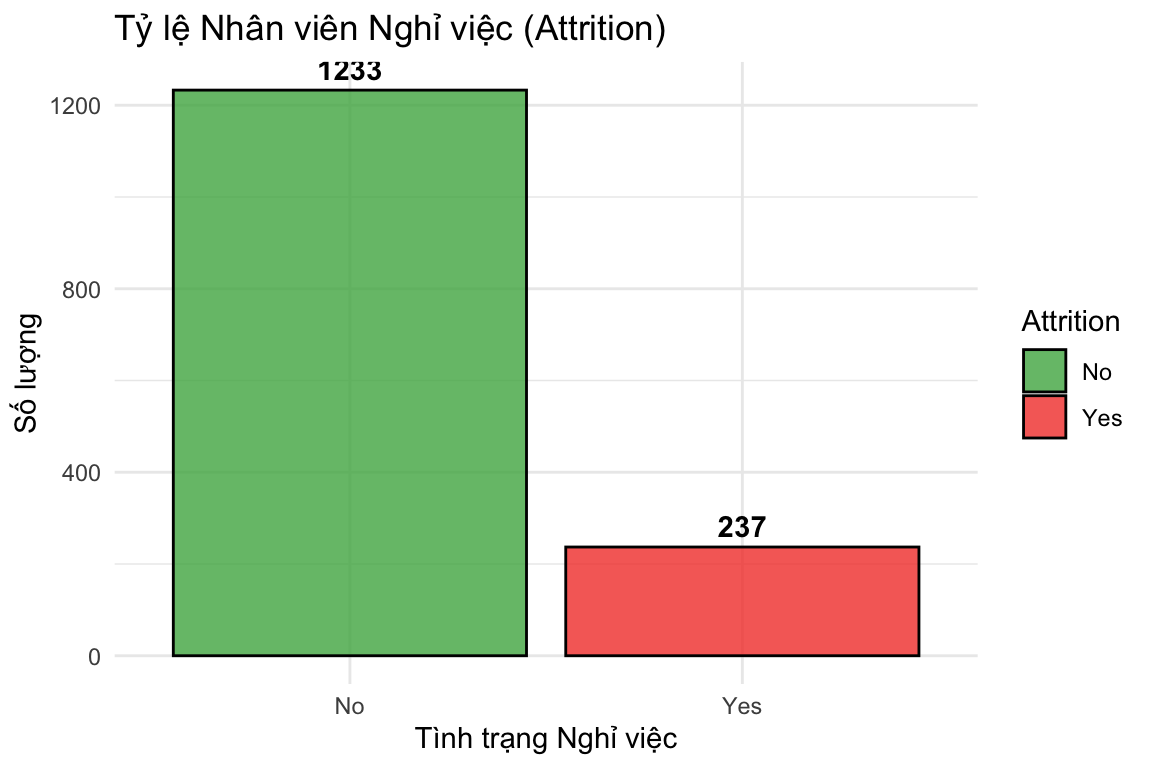
\includegraphics[width=\linewidth,trim=0 20 0 28,clip]
        {img/hr-attrition-distribution.png}
    \end{column}
    \begin{column}{0.41\textwidth}
      \begin{columns}[onlytextwidth]
        \begin{column}{0.48\textwidth}
          \metric{1.470}{nhân viên}{HCMUSBlue}
        \end{column}
        \begin{column}{0.48\textwidth}
          \metric{35}{biến ban đầu}{HCMUSTeal}
        \end{column}
      \end{columns}
      \vspace{0.18cm}
      \begin{beamercolorbox}[sep=0.17cm,rounded=true]{block body}
        \small
        \textbf{Dữ liệu mô phỏng IBM HR Analytics}\\
        Không có giá trị khuyết; loại ba biến hằng và một mã định danh.
      \end{beamercolorbox}
      \vspace{0.18cm}
      \begin{beamercolorbox}[sep=0.17cm,rounded=true]{alerted text}
        \small
        Luôn dự báo ``ở lại'' đã đạt \textbf{83,88\% accuracy},
        nhưng phát hiện \textbf{0\%} ca nghỉ việc.
      \end{beamercolorbox}
      \vspace{0.16cm}
      \centering\small
      $\Rightarrow$ Ưu tiên \textbf{AUC, sensitivity, precision và F1}.
    \end{column}
  \end{columns}
  \vspace{-0.05cm}
  {\tiny\color{MutedText}Nguồn: IBM HR Analytics Employee Attrition \& Performance
  (Kaggle, 2017); dữ liệu mô phỏng.}
\end{frame}



% Thời lượng: 0:45
% Thông điệp: Mục tiêu không phải chỉ đạt accuracy cao, mà là phát hiện sớm
% và chuyển tín hiệu dự báo thành can thiệp có trách nhiệm.
\begin{frame}{Bài toán quản trị: phát hiện sớm, không gắn nhãn}
  \begin{columns}[T,onlytextwidth]
    \begin{column}{0.63\textwidth}
      \vspace{0.12cm}
      \begin{enumerate}
        \item \textbf{Nhận diện chân dung rủi ro}\\
              Ai thường nghỉ việc và tín hiệu nào đáng chú ý?
        \vspace{0.22cm}
        \item \textbf{Dự báo ngoài mẫu}\\
              Mô hình nào cân bằng giữa hiệu suất và khả năng giải thích?
        \vspace{0.22cm}
        \item \textbf{Chuyển thành hành động HR}\\
              Can thiệp vào điều kiện có thể cải thiện, không dùng mô hình
              để tự động ra quyết định bất lợi.
      \end{enumerate}
    \end{column}
    \begin{column}{0.34\textwidth}
      \begin{block}{Biến phản hồi}
        \centering
        \texttt{Attrition}\\[0.08cm]
        \textbf{Yes} = đã nghỉ việc\\
        \textbf{No} = còn làm việc
      \end{block}
      \vspace{0.12cm}
      \begin{beamercolorbox}[sep=0.16cm,rounded=true]{block body}
        \centering\small
        \textbf{Kết quả phản ánh liên hệ dự báo,}\\
        không tự thân chứng minh nhân quả.
      \end{beamercolorbox}
    \end{column}
  \end{columns}
\end{frame}

% Thời lượng: 1:00
% Thông điệp: Toàn cảnh sáu bước đã thực hiện; các slide sau đi đúng trình tự này.
\begin{frame}{Quy trình phân tích: sáu bước đã thực hiện}
  \vspace{0.20cm}
  \centering
  \begin{tikzpicture}[
    pstep/.style={draw=HCMUSBlue,very thick,rounded corners=3pt,
      fill=HCMUSLight,minimum width=4.15cm,minimum height=1.30cm,
      align=center,font=\small},
    arrow/.style={-latex,very thick,draw=HCMUSTeal}
  ]
    \node[pstep] (s1) {\textbf{1. EDA \& thống kê mô tả}\\phân phối, mất cân bằng lớp};
    \node[pstep,right=0.50cm of s1] (s2) {\textbf{2. Kiểm định thống kê}\\Shapiro--Wilk, Wilcoxon, $\chi^2$};
    \node[pstep,right=0.50cm of s2] (s3) {\textbf{3. Chia 70/30 phân tầng}\\tiền xử lý fit trên train};
    \node[pstep,below=0.55cm of s3] (s4) {\textbf{4. Ba mô hình theo tầng}\\logistic $\times 2$ + LASSO};
    \node[pstep,left=0.50cm of s4] (s5) {\textbf{5. Đánh giá trên test}\\AUC, recall, F1; ngưỡng 0,30};
    \node[pstep,left=0.50cm of s5] (s6) {\textbf{6. Diễn giải \& đề xuất}\\odds ratio $\to$ hành động HR};
    \draw[arrow] (s1) -- (s2);
    \draw[arrow] (s2) -- (s3);
    \draw[arrow] (s3) -- (s4);
    \draw[arrow] (s4) -- (s5);
    \draw[arrow] (s5) -- (s6);
  \end{tikzpicture}

  \vspace{0.35cm}
  \begin{beamercolorbox}[sep=0.15cm,rounded=true]{block body}
    \centering\small
    Mỗi bước có kiểm chứng đi kèm: kiểm định giả định trước khi chọn phép kiểm,
    VIF/GVIF cho đa cộng tuyến, 10-fold CV cho $\lambda$,
    và ngưỡng quyết định được khảo sát bằng ba tiêu chí.
  \end{beamercolorbox}
\end{frame}

% SLIDE 7
% Thời lượng: 1:15
% Lời thoại gợi ý: Nhóm nghỉ việc trẻ hơn; đỉnh mật độ 28--31 tuổi.
% Nhân viên độc thân có tỷ lệ nghỉ việc cao gấp khoảng hai lần các nhóm còn lại.
\begin{frame}{Phân tích nhân khẩu học: tuổi và tình trạng hôn nhân}
  \begin{columns}[T,onlytextwidth]
    \begin{column}{0.50\textwidth}
      \centering
      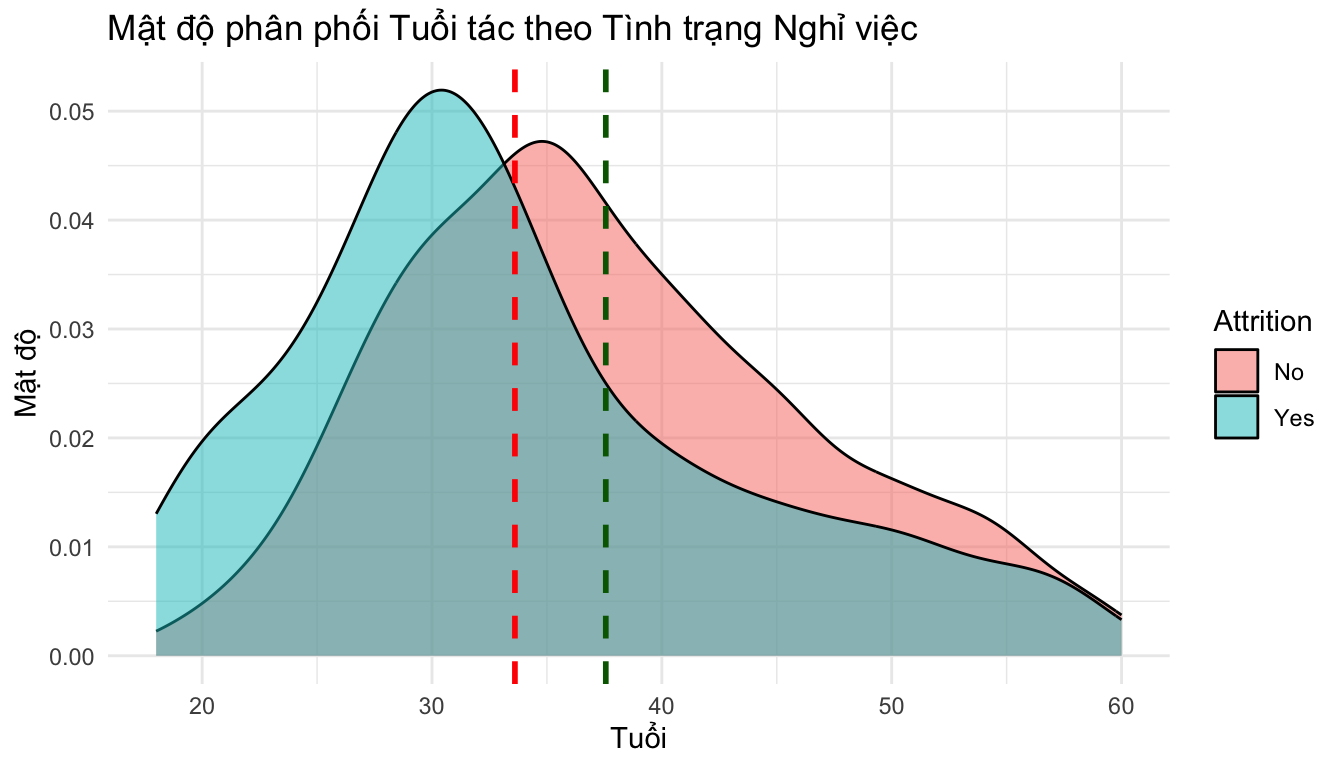
\includegraphics[width=\linewidth,height=4.35cm,keepaspectratio,
        trim=0 18 0 28,clip]{img/hr-age-density.png}\\[-0.04cm]
      \small
      Tuổi trung bình:
      \tagbox{HCMUSRed}{Yes: 33,6}
      \quad \tagbox{HCMUSGreen}{No: 37,6}\\[0.06cm]
      \scriptsize Đỉnh mật độ nghỉ việc tập trung ở nhóm 28--31 tuổi.
    \end{column}
    \begin{column}{0.47\textwidth}
      \centering
      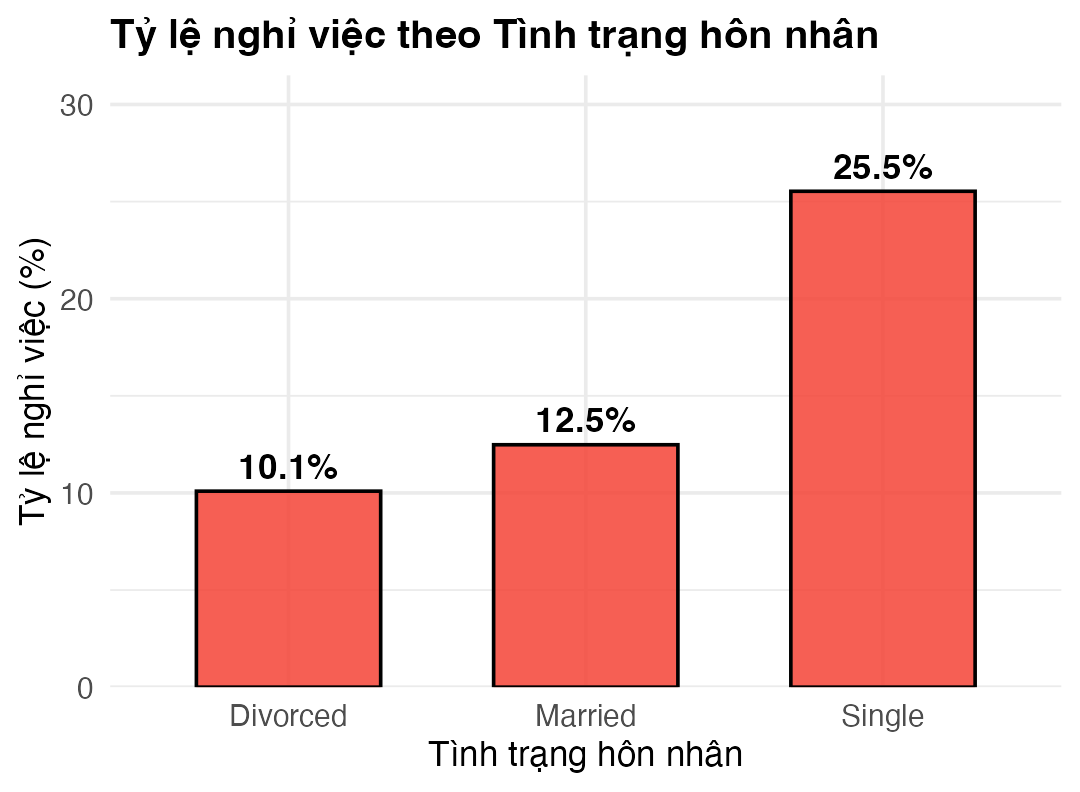
\includegraphics[width=\linewidth,height=4.25cm,keepaspectratio]
        {img/hr-marital-attrition-rate.png}\\[-0.02cm]
      \scriptsize Pearson $\chi^2=46{,}16$, $p<0{,}001$.
    \end{column}
  \end{columns}
  \vspace{0.12cm}
  \begin{beamercolorbox}[sep=0.13cm,rounded=true]{block body}
    \centering\small
    Hồ sơ mô tả ban đầu: nhân sự trẻ và độc thân có tính linh hoạt nghề
    nghiệp cao hơn; đây là \textbf{tín hiệu liên hệ}, không phải nguyên
    nhân hay tiêu chí để tự động đánh giá cá nhân.
  \end{beamercolorbox}
\end{frame}

% SLIDE 8
% Thời lượng: 1:15
% Lời thoại gợi ý: Thu nhập lệch phải nên dùng Wilcoxon; khoảng cách đi làm
% của nhóm nghỉ việc cũng dài hơn có ý nghĩa thống kê.
\begin{frame}{Thu nhập và khoảng cách đi làm}
  \begin{columns}[T,onlytextwidth]
    \begin{column}{0.51\textwidth}
      \centering
      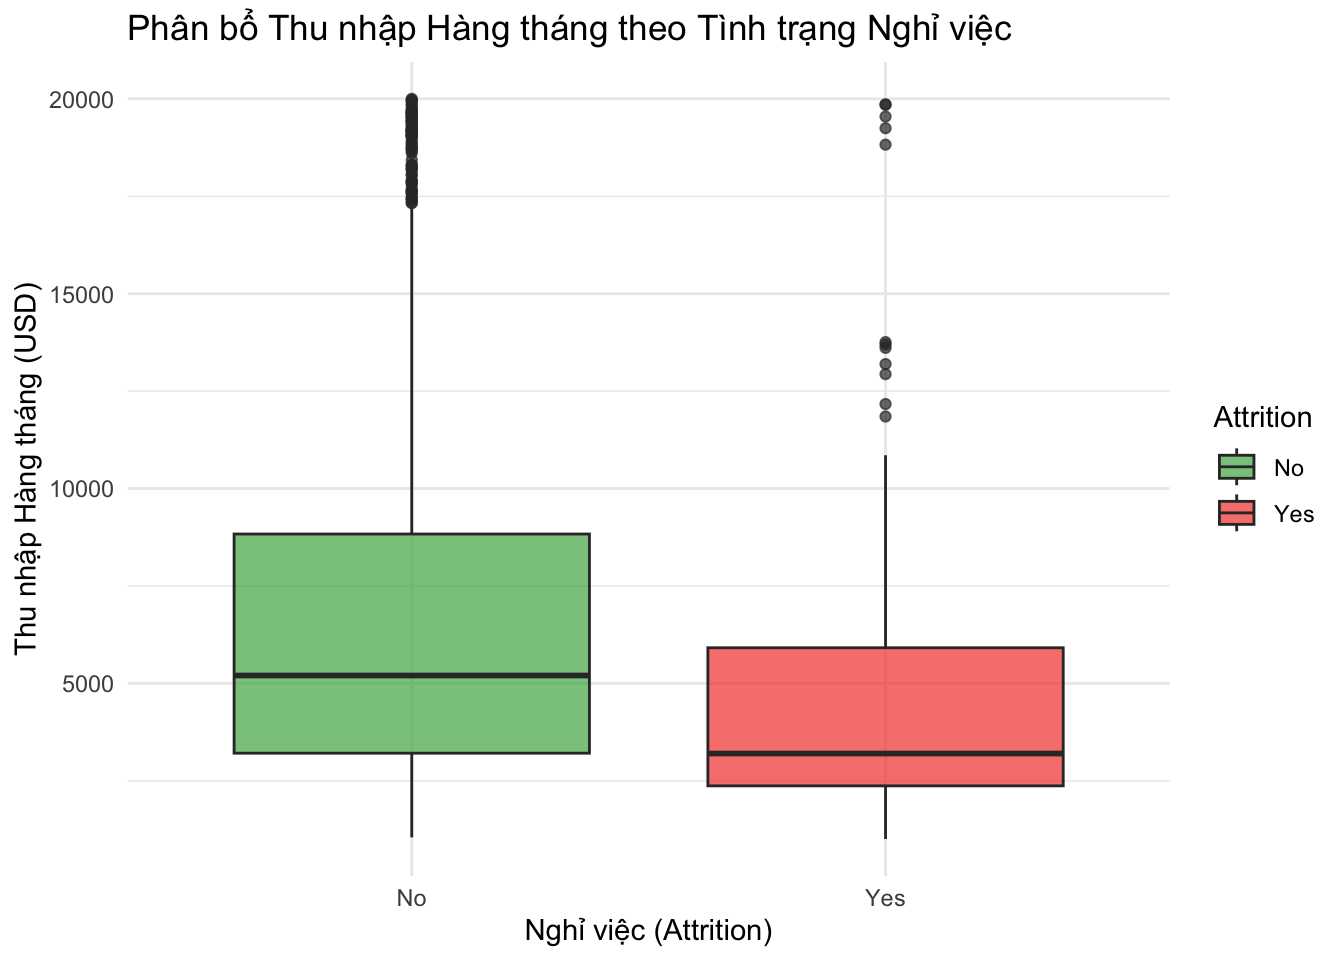
\includegraphics[width=\linewidth,height=4.25cm,keepaspectratio,
        trim=0 28 0 40,clip]{img/hr-income-by-attrition.png}\\[-0.03cm]
      \small
      Trung vị: \tagbox{HCMUSRed}{Yes: 3.202 USD}
      \quad \tagbox{HCMUSGreen}{No: 5.204 USD}\\[0.05cm]
      \scriptsize Wilcoxon: $W=191601$, $p=2{,}95\times10^{-14}$.
    \end{column}
    \begin{column}{0.46\textwidth}
      \centering
      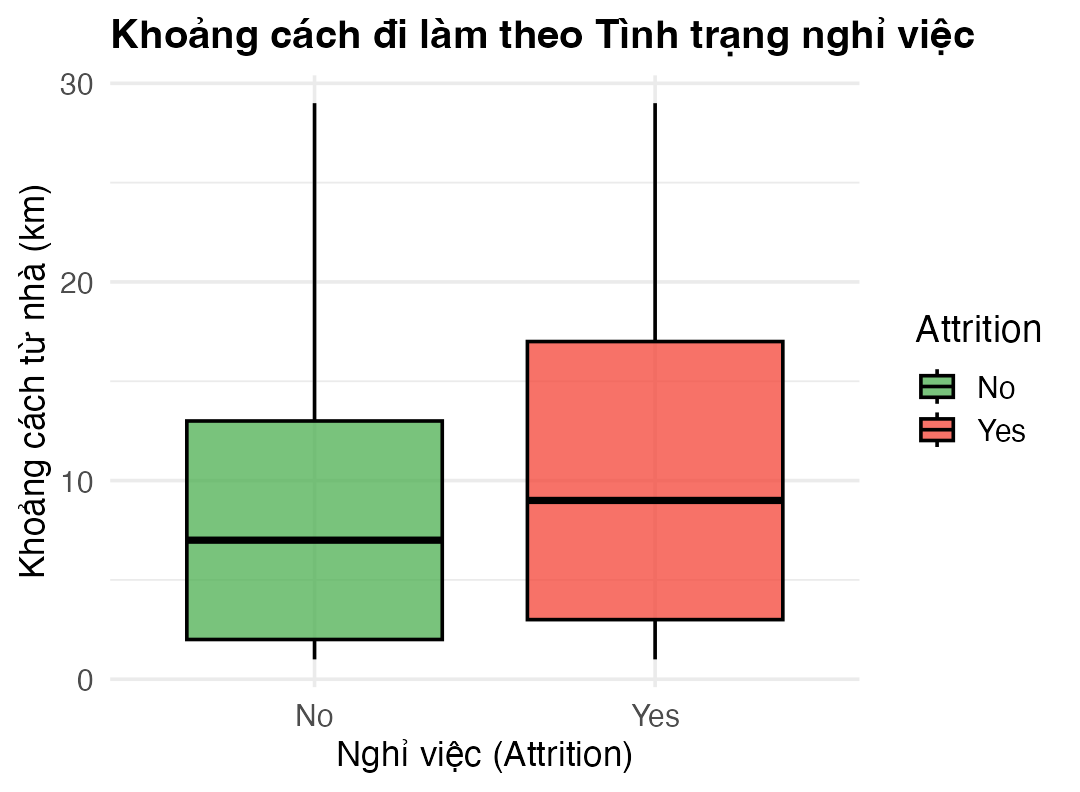
\includegraphics[width=\linewidth,height=4.20cm,keepaspectratio]
        {img/hr-distance-by-attrition.png}\\[-0.02cm]
      \small
      Trung bình: \textbf{10,6} so với \textbf{8,9}.\\[0.04cm]
      \scriptsize Kiểm định $t$ hai mẫu: $p=0{,}0028$.
    \end{column}
  \end{columns}
  \vspace{0.12cm}
  \begin{beamercolorbox}[sep=0.13cm,rounded=true]{block body}
    \centering\small
    Nhóm nghỉ việc có phân phối thu nhập thấp hơn và quãng đường đi làm
    dài hơn. Hai khác biệt này định hướng mô hình đa biến, chưa tự chứng
    minh tiền lương hay khoảng cách là nguyên nhân trực tiếp.
  \end{beamercolorbox}
\end{frame}

% SLIDE 9
% Thời lượng: 1:15
% Lời thoại gợi ý: Làm thêm giờ là tín hiệu cảnh báo mạnh nhất; mức hài lòng
% thấp đi cùng tỷ lệ nghỉ việc cao hơn.
\begin{frame}{Điều kiện công việc: làm thêm giờ và mức độ hài lòng}
  \begin{columns}[T,onlytextwidth]
    \begin{column}{0.45\textwidth}
      \centering
      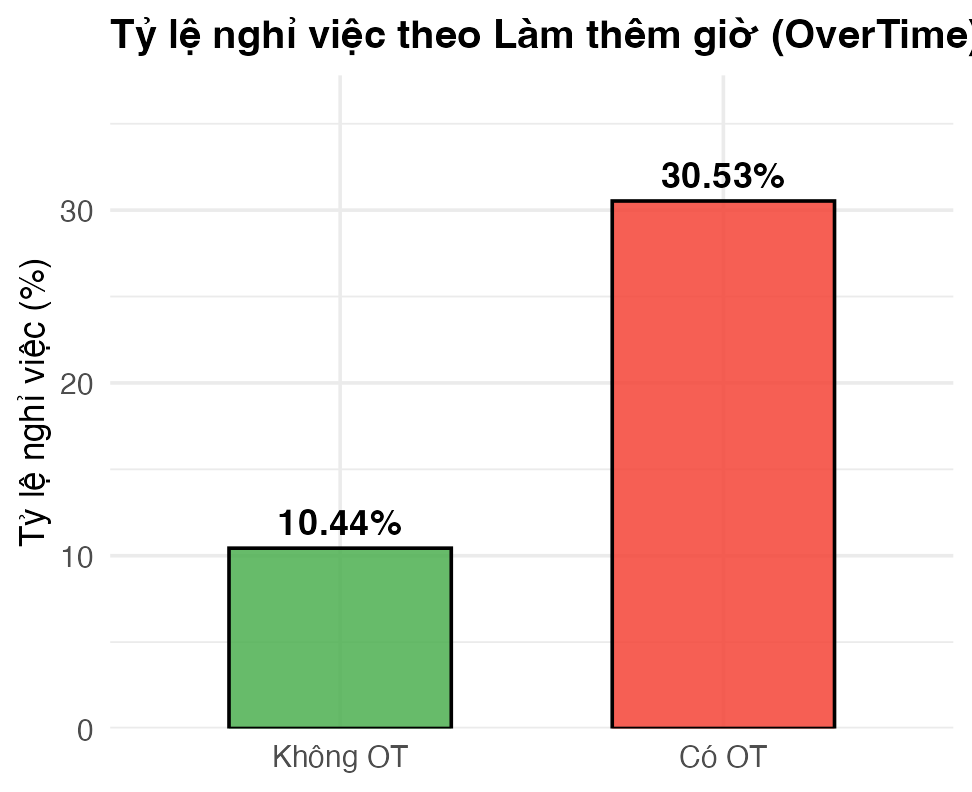
\includegraphics[width=\linewidth,height=4.35cm,keepaspectratio]
        {img/hr-overtime-attrition-rate.png}\\[-0.03cm]
      \scriptsize Pearson $\chi^2=87{,}56$, $p<0{,}001$.
    \end{column}
    \begin{column}{0.52\textwidth}
      \centering
      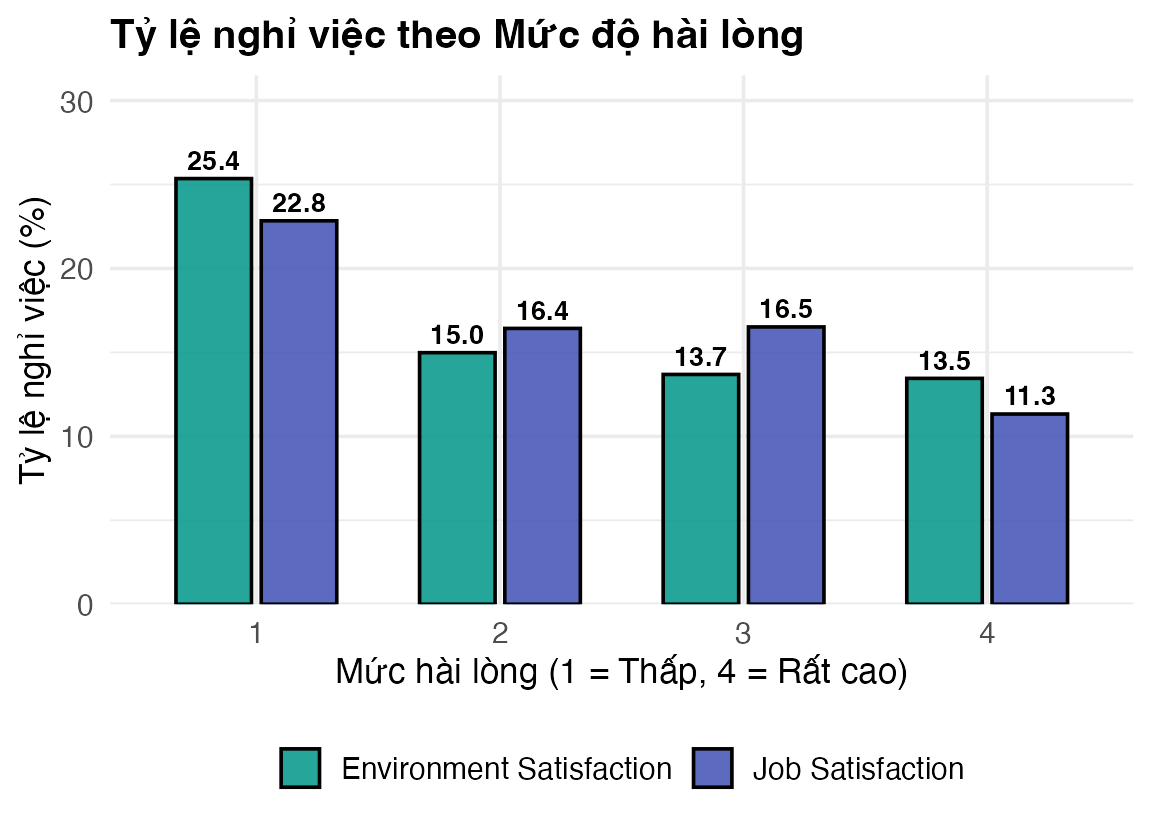
\includegraphics[width=\linewidth,height=4.35cm,keepaspectratio]
        {img/hr-satisfaction-attrition-rate.png}\\[-0.03cm]
      \scriptsize
      Mức 1: Job Satisfaction \textbf{22,84\%};
      Environment Satisfaction \textbf{25,35\%}.
    \end{column}
  \end{columns}
  \vspace{0.10cm}
  \begin{beamercolorbox}[sep=0.13cm,rounded=true]{alerted text}
    \centering\small
    Có OT: \textbf{30,53\%} nghỉ việc; không OT: \textbf{10,44\%}.
    Tỷ lệ cao gần gấp ba lần, trong khi hài lòng thấp cũng đi cùng rủi ro
    lớn hơn --- đây là các yếu tố doanh nghiệp có thể can thiệp.
  \end{beamercolorbox}
\end{frame}

% SLIDE 10
% Thời lượng: 1:15
% Lời thoại gợi ý: Phân biệt số người nghỉ tuyệt đối với tỷ lệ nghỉ; đi sâu
% xuống chức danh cho thấy Sales Representative là điểm nóng lớn nhất.
\begin{frame}{Phòng ban và chức danh có tỷ lệ nghỉ việc cao}
  \begin{columns}[T,onlytextwidth]
    \begin{column}{0.47\textwidth}
      \centering
      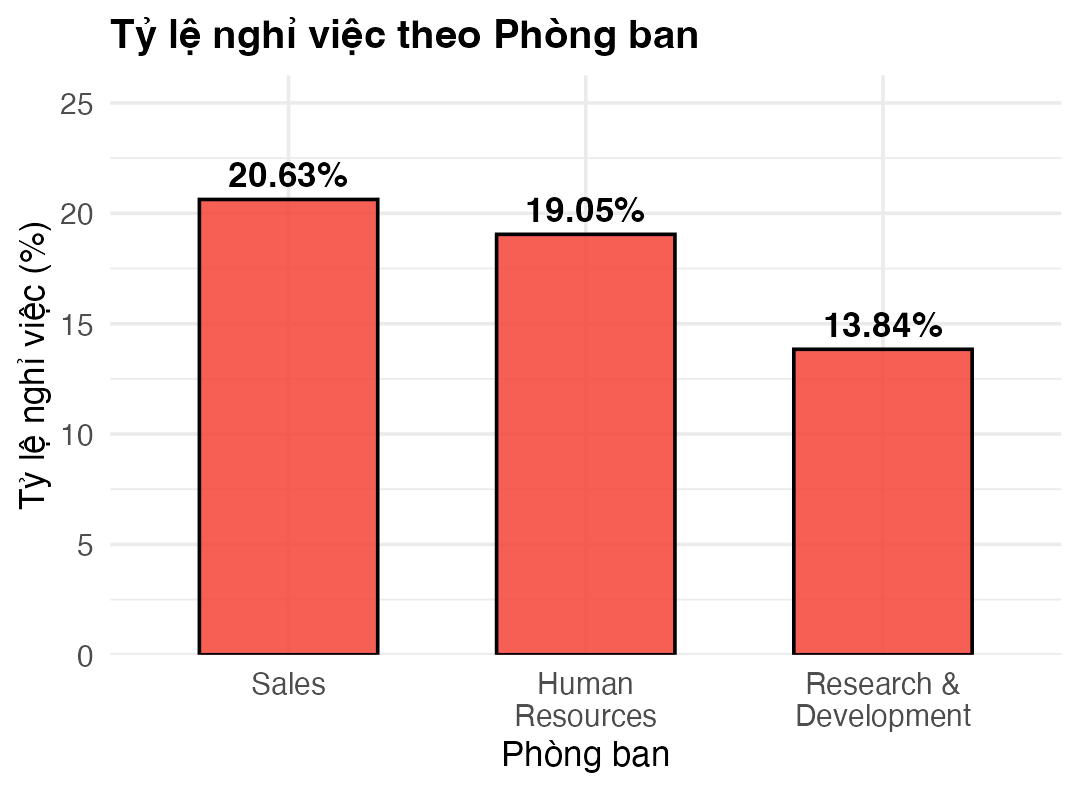
\includegraphics[width=\linewidth,height=4.35cm,keepaspectratio]
        {img/hr-department-attrition-rate.png}\\[-0.03cm]
      \scriptsize Pearson $\chi^2=10{,}80$, $p=0{,}0045$.
    \end{column}
    \begin{column}{0.50\textwidth}
      \centering
      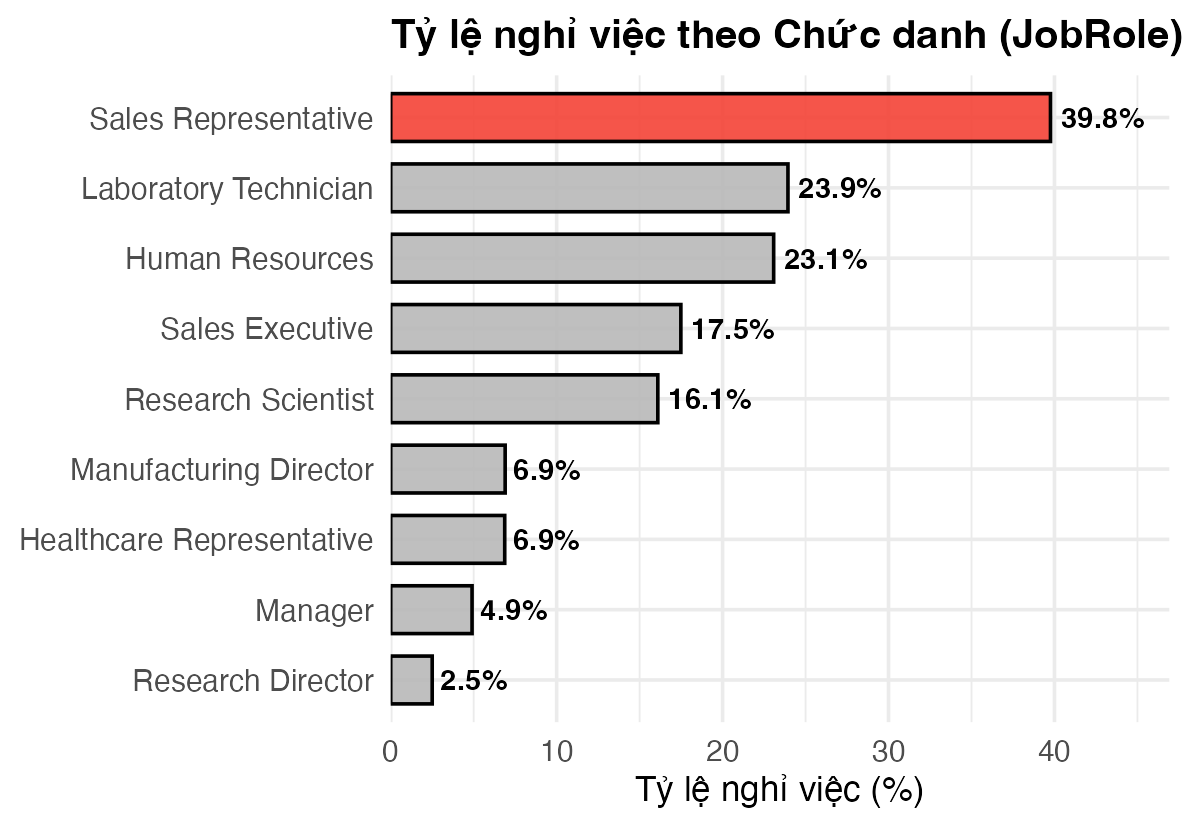
\includegraphics[width=\linewidth,height=4.35cm,keepaspectratio]
        {img/hr-jobrole-risk.png}
    \end{column}
  \end{columns}
  \vspace{0.08cm}
  \begin{beamercolorbox}[sep=0.13cm,rounded=true]{block body}
    \centering\small
    Chân dung rủi ro từ EDA: nhân sự trẻ, độc thân, thuộc Sales hoặc các
    vai trò Sales Representative/Laboratory Technician/HR, thường làm OT
    và có thu nhập thấp hơn. Hồ sơ này chỉ dùng để định hướng mô hình và
    khảo sát giữ chân.
  \end{beamercolorbox}
\end{frame}

% Thời lượng: 1:00
% Thông điệp: Bốn quyết định tiền xử lý chính trước khi mô hình hóa;
% mọi tham số đều được fit lại chỉ trên train (chi tiết ở slide sau).
\begin{frame}{Tiền xử lý dữ liệu: bốn quyết định chính}
  \begin{columns}[T,onlytextwidth]
    \begin{column}{0.48\textwidth}
      \begin{beamercolorbox}[sep=0.16cm,rounded=true]{block body}
        \textbf{1. Loại biến không mang thông tin}\\[0.04cm]
        \small Ba biến hằng (\texttt{EmployeeCount}, \texttt{Over18},
        \texttt{StandardHours}) và mã định danh \texttt{EmployeeNumber}
        --- phương sai bằng 0, không có giá trị dự báo.
      \end{beamercolorbox}
      \vspace{0.16cm}
      \begin{beamercolorbox}[sep=0.16cm,rounded=true]{block body}
        \textbf{2. Dữ liệu khuyết: không có}\\[0.04cm]
        \small 0 giá trị NA trên toàn bộ 1.470 quan sát
        $\Rightarrow$ không cần các phép gán thay thế (imputation).
      \end{beamercolorbox}
    \end{column}
    \begin{column}{0.48\textwidth}
      \begin{beamercolorbox}[sep=0.16cm,rounded=true]{block body}
        \textbf{3. Giới hạn ngoại lệ thu nhập}\\[0.04cm]
        \small \texttt{MonthlyIncome} lệch phải (trung bình 6.503 $>$
        trung vị 4.919 USD): capping tại $Q_1-1{,}5\,\mathrm{IQR}$ và
        $Q_3+1{,}5\,\mathrm{IQR}$ thay vì xóa quan sát.
      \end{beamercolorbox}
      \vspace{0.16cm}
      \begin{beamercolorbox}[sep=0.16cm,rounded=true]{block body}
        \textbf{4. Chuẩn hóa và mã hóa}\\[0.04cm]
        \small Z-score cho tuổi và thu nhập; biến phân loại dummy hóa
        full rank ($K-1$ cột, có nhóm tham chiếu).
      \end{beamercolorbox}
    \end{column}
  \end{columns}
  \vspace{0.20cm}
  \begin{beamercolorbox}[sep=0.15cm,rounded=true]{alerted text}
    \centering\small
    Mọi tham số tiền xử lý (ngưỡng capping, $\mu$, $\sigma$, bộ mã hóa dummy)
    đều được \textbf{fit lại chỉ trên tập train} --- thiết kế chống rò rỉ
    ở slide tiếp theo.
  \end{beamercolorbox}
\end{frame}

% Thời lượng: 1:00
% Thông điệp: Mọi bước học từ phân phối đều chỉ fit trên train; test chỉ dùng
% để đánh giá ngoài mẫu, có stopifnot kiểm chứng tự động.
\begin{frame}{Thiết kế đánh giá ngoài mẫu, hạn chế rò rỉ dữ liệu}
  \vspace{0.25cm}
  \centering
  \begin{tikzpicture}[
    box/.style={draw=HCMUSBlue,very thick,rounded corners=3pt,
      fill=HCMUSLight,minimum width=2.45cm,minimum height=1.15cm,
      align=center,font=\small},
    arrow/.style={-latex,very thick,draw=HCMUSTeal}
  ]
    \node[box] (data) {\textbf{1.470 quan sát}\\chia phân tầng 70/30};
    \node[box,right=0.65cm of data] (prep) {\textbf{Tiền xử lý trên train}\\IQR capping, chuẩn hóa,\\one-hot encoding };
    \node[box,right=0.65cm of prep] (models) {\textbf{Huấn luyện}\\2 Logistic + LASSO};
    \node[box,right=0.65cm of models] (test) {\textbf{Đánh giá test}\\AUC, recall, F1};
    \draw[arrow] (data) -- (prep);
    \draw[arrow] (prep) -- (models);
    \draw[arrow] (models) -- (test);
  \end{tikzpicture}

  \vspace{0.45cm}
  \begin{columns}[T,onlytextwidth]
    \begin{column}{0.31\textwidth}
      \metric{1.030}{tập huấn luyện}{HCMUSBlue}
    \end{column}
    \begin{column}{0.31\textwidth}
      \metric{440}{tập kiểm thử}{HCMUSTeal}
    \end{column}
    \begin{column}{0.31\textwidth}
      \metric{10-fold}{CV chọn $\lambda$ LASSO}{HCMUSRed}
    \end{column}
  \end{columns}

\end{frame}

\begin{frame}{Ba đặc tả hồi quy logistic được so sánh}
  \begin{columns}[T,onlytextwidth]
    \begin{column}{0.31\textwidth}
      \begin{block}{1. Nhân khẩu học}
        \small
        \textbf{Biến:} tuổi, giới tính, hôn nhân, khoảng cách, học vấn.\\[0.14cm]
        \textbf{AUC test:} 0,656
      \end{block}
    \end{column}
    \begin{column}{0.31\textwidth}
      \begin{block}{2. Công việc}
        \small
        \textbf{Biến:} chức danh, hài lòng, làm thêm giờ, thu nhập.\\[0.14cm]
        \textbf{AUC test:} 0,785
      \end{block}
    \end{column}
    \begin{column}{0.31\textwidth}
      \begin{block}{3. LASSO (phạt $L_1$)}
        \small
        \textbf{Biến:} toàn bộ 30 biến gốc; giữ 35 hệ số $\neq 0$.\\[0.14cm]
        \textbf{AUC test:} \textbf{0,854}
      \end{block}
    \end{column}
  \end{columns}
  \vspace{0.22cm}
  \begin{beamercolorbox}[sep=0.14cm,rounded=true]{block body}
    \centering\small
    Cùng biến phản hồi $Y_i=1$ nếu nhân viên nghỉ việc, cả ba mô hình hóa
    $p_i=P(Y_i=1\mid\mathbf{x}_i)$:
    $\displaystyle \log\!\left(\frac{p_i}{1-p_i}\right)
      =\beta_0+\sum_j\beta_jx_{ij}$.
  \end{beamercolorbox}
\end{frame}

\begin{frame}{Công thức của hai mô hình logistic không phạt}
  \small
  Đặt $p_i=P(\texttt{Attrition}_i=\texttt{Yes}\mid\mathbf{x}_i)$ và
  $\operatorname{logit}(p_i)=\log[p_i/(1-p_i)]$.
  \vspace{0.12cm}
  \begin{block}{Mô hình 1: nhân khẩu học}
    \[
      \operatorname{logit}(p_i)=\beta_0+\beta_1\text{AgeScaled}_i
      +\boldsymbol\beta_2^{\top}\text{Gender}_i
      +\boldsymbol\beta_3^{\top}\text{MaritalStatus}_i
      +\beta_4\text{Distance}_i+\beta_5\text{Education}_i.
    \]
  \end{block}
  \vspace{0.08cm}
  \begin{block}{Mô hình 2: công việc và môi trường}
    \[
      \begin{aligned}
      \operatorname{logit}(p_i)={}&\alpha_0
      +\boldsymbol\alpha_1^{\top}\text{JobRole}_i
      +\alpha_2\text{EnvironmentSatisfaction}_i\\
      &+\alpha_3\text{JobSatisfaction}_i
      +\alpha_4\text{OverTime}_i
      +\alpha_5\text{IncomeScaled}_i.
      \end{aligned}
    \]
  \end{block}
  \vspace{0.05cm}
  {\scriptsize\color{MutedText}
    Chữ đậm biểu thị một nhóm hệ số dummy. Nhóm tham chiếu lần lượt gồm
    nữ, đã ly hôn, Healthcare Representative và không làm thêm giờ.}
\end{frame}

% Thời lượng: 0:45
% Thông điệp: Chiếu output thật của đặc tả đầu — người nghe tự thấy các
% con số dị dạng (dòng tô nền) trước khi slide sau đưa ra chẩn đoán.
\begin{frame}{Kết quả đặc tả đầu: mô hình công việc còn \texttt{Department}}
  \centering\tiny
  \renewcommand{\arraystretch}{1.02}
  \begin{tabular}{lrrrr}
    \toprule
    \textbf{Biến} & $\hat\alpha$ & \textbf{SE} & $z$ & $p$\\
    \midrule
    \rowcolor{HCMUSLight}
    Hằng số & $-14{,}89$ & $954{,}6$ & $-0{,}016$ & $0{,}988$\\
    \rowcolor{HCMUSLight}
    Department: Research \& Development & $13{,}43$ & $954{,}6$ & $0{,}014$ & $0{,}989$\\
    \rowcolor{HCMUSLight}
    Department: Sales & $-0{,}2340$ & $1.082{,}0$ & $0{,}000$ & $0{,}9998$\\
    \rowcolor{HCMUSLight}
    JobRole: Human Resources & $14{,}83$ & $954{,}6$ & $0{,}016$ & $0{,}988$\\
    JobRole: Laboratory Technician & $1{,}6410$ & $0{,}5027$ & $3{,}264$ & $0{,}001$\\
    JobRole: Manager & $-0{,}4037$ & $0{,}9284$ & $-0{,}435$ & $0{,}664$\\
    JobRole: Manufacturing Director & $0{,}1588$ & $0{,}5439$ & $0{,}290$ & $0{,}770$\\
    JobRole: Research Director & $-1{,}6270$ & $1{,}1540$ & $-1{,}403$ & $0{,}159$\\
    JobRole: Research Scientist & $0{,}7135$ & $0{,}5156$ & $1{,}384$ & $0{,}166$\\
    \rowcolor{HCMUSLight}
    JobRole: Sales Executive & $14{,}64$ & $510{,}1$ & $0{,}029$ & $0{,}977$\\
    \rowcolor{HCMUSLight}
    JobRole: Sales Representative & $15{,}92$ & $510{,}1$ & $0{,}031$ & $0{,}975$\\
    Hài lòng môi trường & $-0{,}3613$ & $0{,}0866$ & $-4{,}172$ & $<0{,}001$\\
    Hài lòng công việc & $-0{,}2813$ & $0{,}0831$ & $-3{,}384$ & $<0{,}001$\\
    Làm thêm giờ & $1{,}5420$ & $0{,}1950$ & $7{,}908$ & $<0{,}001$\\
    Thu nhập chuẩn hóa & $-0{,}0039$ & $0{,}2135$ & $-0{,}018$ & $0{,}986$\\
    \bottomrule
  \end{tabular}
  \vspace{0.16cm}
  \begin{beamercolorbox}[sep=0.11cm,rounded=true]{block body}
    \scriptsize
    Nguồn: \texttt{summary(model\_2)} của đặc tả có \texttt{Department}
    (mục 2.3 báo cáo); Fisher scoring: \textbf{15 vòng} (bình thường 5--6).
    Các dòng tô nền có hệ số và sai số chuẩn bất thường trong khi các biến
    còn lại vẫn lành mạnh --- chẩn đoán ở slide tiếp theo.
  \end{beamercolorbox}
\end{frame}


% Thời lượng: 1:15
% Thông điệp: Trình bày lỗi đã gặp và cách chẩn đoán -- điểm cộng quy trình:
% phiên bản đầu của mô hình công việc suy biến vì Department lồng trong JobRole.
\begin{frame}{Chẩn đoán đa cộng tuyến cấu trúc ở mô hình công việc}
  \begin{columns}[T,onlytextwidth]
    \begin{column}{0.48\textwidth}
      \begin{beamercolorbox}[sep=0.16cm,rounded=true]{block body}
        \textbf{\color{HCMUSRed}Dấu hiệu bất thường trong output}\\[0.04cm]
        \small
        $\beta \approx 13$--$16$: OR hàng triệu lần, phi thực tế.\\
        SE $\approx 510$--$1.082$: CI chứa mọi giá trị.\\
        $p \to 1$ ở chính các biến quan trọng.\\
        Fisher scoring 15 vòng (bình thường 5--6).
      \end{beamercolorbox}
      \vspace{0.16cm}
      \begin{beamercolorbox}[sep=0.16cm,rounded=true]{block body}
        \textbf{Nguyên nhân}\\[0.04cm]
        \small
        \texttt{Department} lồng trong \texttt{JobRole}:
        mọi Sales Executive đều thuộc Sales
        $\Rightarrow$ thông tin trùng lặp gần hoàn hảo.
      \end{beamercolorbox}
    \end{column}
    \begin{column}{0.48\textwidth}
      \begin{beamercolorbox}[sep=0.16cm,rounded=true]{block body}
        \textbf{\color{HCMUSGreen}Xử lý}\\[0.04cm]
        \small
        Loại \texttt{Department}, giữ \texttt{JobRole}
        --- biến chi tiết hơn, đã bao phủ thông tin phòng ban.
      \end{beamercolorbox}
      \vspace{0.16cm}
      \begin{beamercolorbox}[sep=0.16cm,rounded=true]{block body}
        \textbf{Sau khi sửa}\\[0.04cm]
        \small
        Hội tụ sau 6 vòng; AIC 783,18 $\to$ 781,32;
        GVIF lớn nhất $\approx 2{,}94 < 5$.
      \end{beamercolorbox}
    \end{column}
  \end{columns}
  \vspace{0.18cm}
  {\scriptsize\color{MutedText}
   Mô hình nhân khẩu học cũng được kiểm tra tương tự: GVIF lớn nhất
   $\approx 1{,}10$. Bảng VIF/GVIF đầy đủ ở phần backup.}
\end{frame}

% Thời lượng: 0:45
% Thông điệp: Bằng chứng định lượng cho việc loại Department -- GVIF quy đổi
% của mô hình công việc từ hàng triệu về 2,82, dưới ngưỡng tham khảo 5.
\begin{frame}{GVIF mô hình công việc: trước và sau khi loại \texttt{Department}}
  \begin{columns}[T,onlytextwidth]
    \begin{column}{0.49\textwidth}
      \centering\small
      \textbf{\color{HCMUSRed}Trước: có \texttt{Department}}\\[0.12cm]
      \scriptsize
      \renewcommand{\arraystretch}{1.22}
      \begin{tabular}{lrr}
        \toprule
        Biến & VIF & GVIF\\
        \midrule
        \rowcolor{HCMUSLight}
        Department & --- & $\mathbf{3{,}8{\times}10^{13}}$\\
        \rowcolor{HCMUSLight}
        JobRole & --- & $\mathbf{1{,}1{\times}10^{14}}$\\
        EnvironmentSatisfaction & 1,042 & 1,042\\
        JobSatisfaction & 1,014 & 1,014\\
        OverTime & 1,088 & 1,088\\
        Income\_scaled & 2,772 & 2,772\\
        \bottomrule
      \end{tabular}
    \end{column}
    \begin{column}{0.49\textwidth}
      \centering\small
      \textbf{\color{HCMUSGreen}Sau: đã loại \texttt{Department}}\\[0.12cm]
      \scriptsize
      \renewcommand{\arraystretch}{1.22}
      \begin{tabular}{lrr}
        \toprule
        Biến & VIF & GVIF\\
        \midrule
        JobRole & --- & \textbf{2,935}\\
        EnvironmentSatisfaction & 1,042 & 1,042\\
        JobSatisfaction & 1,013 & 1,013\\
        OverTime & 1,090 & 1,090\\
        Income\_scaled & 2,816 & 2,816\\
        & & \\
        \bottomrule
      \end{tabular}
    \end{column}
  \end{columns}
  \vspace{0.20cm}
  \begin{beamercolorbox}[sep=0.14cm,rounded=true]{block body}
    \centering\small
    Giá trị lớn nhất giảm từ cỡ $10^{14}$ xuống \textbf{2,94}, dưới ngưỡng
    tham khảo \textbf{5}. Các biến không liên quan hầu như không đổi ---
    cộng tuyến khu trú đúng cặp \texttt{Department}--\texttt{JobRole}.
  \end{beamercolorbox}
  \vspace{0.10cm}
  {\scriptsize\color{MutedText}
   \centering VIF chỉ định nghĩa cho biến một bậc tự do (khi đó GVIF trùng
   VIF); biến phân loại nhiều mức phải dùng GVIF.\par}
\end{frame}


% B8: bảng hệ số đầy đủ của mô hình logistic nhân khẩu học.
\begin{frame}{Kết quả hồi quy logistic nhân khẩu học}
  \centering\scriptsize
  \renewcommand{\arraystretch}{1.16}
  \begin{tabular}{lrrrr}
    \toprule
    \textbf{Biến} & $\hat\beta$ & \textbf{SE} & $z$ & $p$\\
    \midrule
    Hằng số & $-2{,}4969$ & $0{,}3718$ & $-6{,}716$ & $<0{,}001$\\
    Tuổi chuẩn hóa & $-0{,}3905$ & $0{,}0983$ & $-3{,}972$ & $<0{,}001$\\
    Nam & $0{,}2795$ & $0{,}1827$ & $1{,}529$ & $0{,}126$\\
    Đã kết hôn & $-0{,}1142$ & $0{,}2558$ & $-0{,}446$ & $0{,}655$\\
    Độc thân & $0{,}9057$ & $0{,}2441$ & $3{,}710$ & $<0{,}001$\\
    Khoảng cách từ nhà & $0{,}0304$ & $0{,}0104$ & $2{,}932$ & $0{,}003$\\
    Học vấn & $0{,}0021$ & $0{,}0887$ & $0{,}024$ & $0{,}981$\\
    \bottomrule
  \end{tabular}
  \vspace{0.28cm}
  \begin{beamercolorbox}[sep=0.14cm,rounded=true]{block body}
    \small
    $\mathrm{AIC}=858{,}89$; AUC test $=0{,}656$.
    Ở mức 5\%, tuổi, độc thân và khoảng cách từ nhà có hệ số khác 0;
    đây là liên hệ có điều kiện, không phải quan hệ nhân quả.
  \end{beamercolorbox}
\end{frame}

% B9: bảng hệ số đầy đủ của mô hình logistic công việc sau khi loại Department.
\begin{frame}{Kết quả logistic công việc và môi trường}
  \centering\tiny
  \renewcommand{\arraystretch}{1.02}
  \begin{tabular}{lrrrr}
    \toprule
    \textbf{Biến} & $\hat\alpha$ & \textbf{SE} & $z$ & $p$\\
    \midrule
    Hằng số & $-1{,}4438$ & $0{,}5113$ & $-2{,}824$ & $0{,}005$\\
    Human Resources & $1{,}3988$ & $0{,}5932$ & $2{,}358$ & $0{,}018$\\
    Laboratory Technician & $1{,}6364$ & $0{,}5028$ & $3{,}255$ & $0{,}001$\\
    Manager & $-0{,}9600$ & $0{,}9165$ & $-1{,}047$ & $0{,}295$\\
    Manufacturing Director & $0{,}1578$ & $0{,}5439$ & $0{,}290$ & $0{,}772$\\
    Research Director & $-1{,}6197$ & $1{,}1541$ & $-1{,}403$ & $0{,}160$\\
    Research Scientist & $0{,}7086$ & $0{,}5157$ & $1{,}374$ & $0{,}169$\\
    Sales Executive & $0{,}9770$ & $0{,}4471$ & $2{,}185$ & $0{,}029$\\
    Sales Representative & $2{,}2515$ & $0{,}5613$ & $4{,}011$ & $<0{,}001$\\
    Hài lòng môi trường & $-0{,}3619$ & $0{,}0866$ & $-4{,}180$ & $<0{,}001$\\
    Hài lòng công việc & $-0{,}2847$ & $0{,}0832$ & $-3{,}424$ & $0{,}001$\\
    Làm thêm giờ & $1{,}5420$ & $0{,}1951$ & $7{,}904$ & $<0{,}001$\\
    Thu nhập chuẩn hóa & $-0{,}0086$ & $0{,}2138$ & $-0{,}040$ & $0{,}968$\\
    \bottomrule
  \end{tabular}
  \vspace{0.16cm}
  \begin{beamercolorbox}[sep=0.11cm,rounded=true]{block body}
    \scriptsize
    $\mathrm{AIC}=781{,}32$; AUC test $=0{,}785$.
    Nhóm tham chiếu của \texttt{JobRole} là Healthcare Representative;
    \texttt{Department} đã bị loại do phụ thuộc cấu trúc với \texttt{JobRole}.
  \end{beamercolorbox}
\end{frame}


% Thời lượng: 1:00
% Thông điệp: LASSO không phải hộp đen: lambda chọn bằng 10-fold CV,
% có đối chứng lambda.1se đơn giản hơn.
\begin{frame}{LASSO: chọn $\lambda$ bằng 10-fold cross-validation}
  \begin{columns}[T,onlytextwidth]
    \begin{column}{0.55\textwidth}
      \centering
      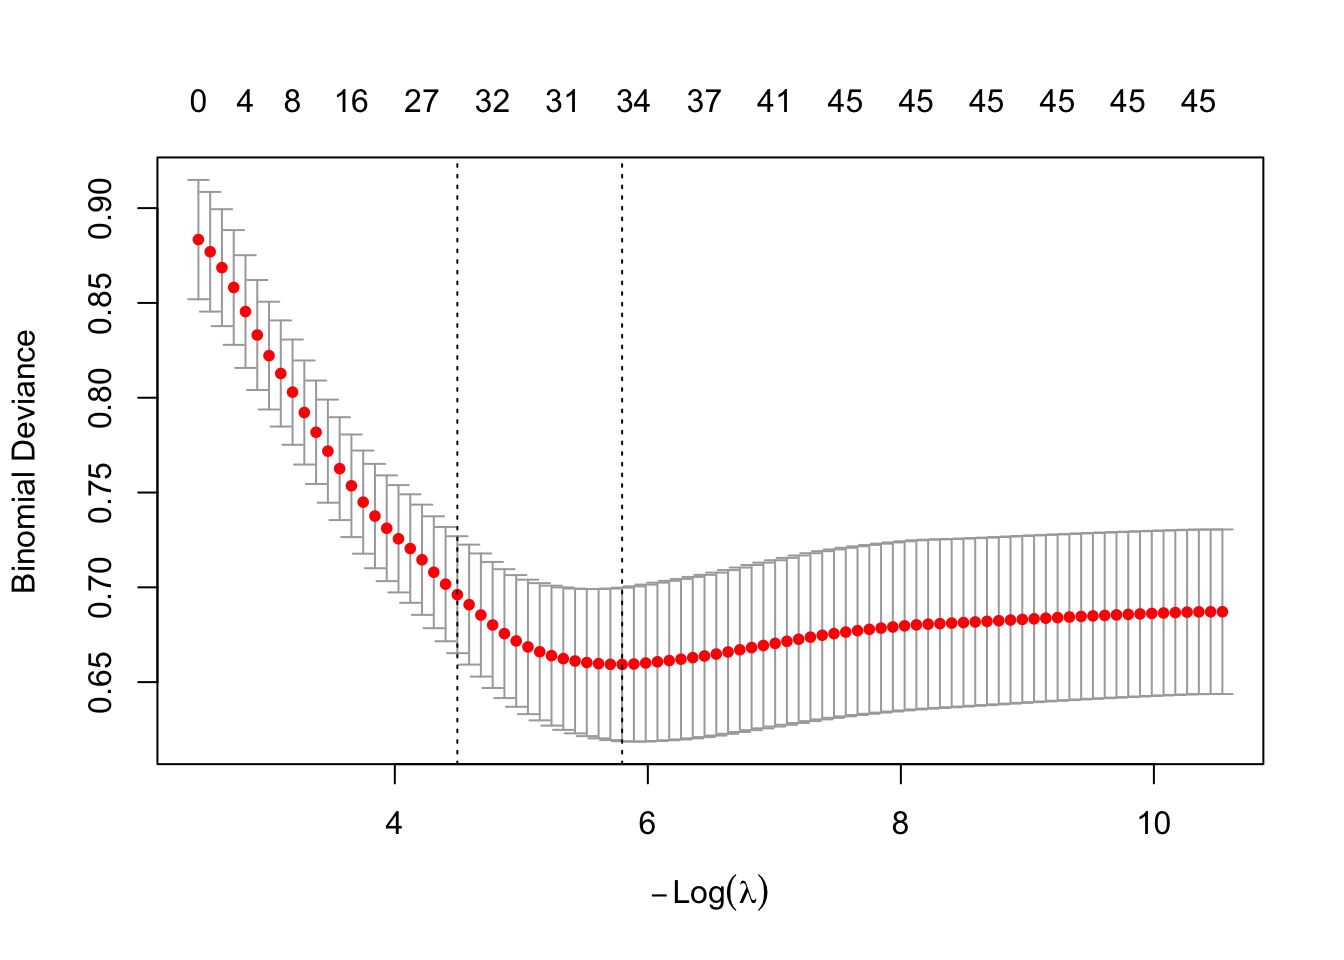
\includegraphics[width=\linewidth,height=5.35cm,keepaspectratio]
        {img/hr-lasso-cv.png}
    \end{column}
    \begin{column}{0.42\textwidth}
      \begin{beamercolorbox}[sep=0.16cm,rounded=true]{block body}
        \centering
        \textbf{\color{HCMUSRed}$\lambda_{\min} \approx 0{,}0030$}\\
        \small $\log\lambda \approx -5{,}80$; giữ \textbf{35 hệ số} $\neq 0$.\\
        Dùng cho mọi dự báo: ưu tiên sai số CV nhỏ nhất.
      \end{beamercolorbox}
      \vspace{0.16cm}
      \begin{beamercolorbox}[sep=0.16cm,rounded=true]{block body}
        \centering
        \textbf{\color{HCMUSTeal}$\lambda_{1se}$}\\
        \small $\log\lambda \approx -4{,}49$; còn \textbf{29 biến}.\\
        Đối chứng gọn hơn nếu ưu tiên triển khai đơn giản.
      \end{beamercolorbox}
      \vspace{0.16cm}
      \small
      Lí do nhóm chọn Lasso: Ma trận dummy lớn; tuổi, thâm niên, cấp bậc, thu nhập
      tương quan --- phạt L1 vừa co hệ số vừa chọn biến.
    \end{column}
  \end{columns}
\end{frame}

% Thời lượng: 1:15
% Thông điệp: Điều kiện công việc có tín hiệu mạnh hơn nhân khẩu học.
% Các OR ở đây đến từ logistic công việc, không phải hệ số LASSO.
\begin{frame}{Yếu tố công việc cung cấp tín hiệu mạnh nhất}
  \begin{columns}[T,onlytextwidth]
    \begin{column}{0.57\textwidth}
      \begin{beamercolorbox}[sep=0.17cm,rounded=true]{block body}
        \textbf{\color{HCMUSRed}Làm thêm giờ}\\[-0.02cm]
        Odds nghỉ việc cao gấp \textbf{4,67 lần}.
      \end{beamercolorbox}
      \vspace{0.16cm}
      \begin{beamercolorbox}[sep=0.17cm,rounded=true]{block body}
        \textbf{\color{HCMUSGreen}Hài lòng môi trường}\\[-0.02cm]
        Tăng một bậc $\Rightarrow$ odds giảm \textbf{30,3\%}.
      \end{beamercolorbox}
      \vspace{0.16cm}
      \begin{beamercolorbox}[sep=0.17cm,rounded=true]{block body}
        \textbf{\color{HCMUSGreen}Hài lòng công việc}\\[-0.02cm]
        Tăng một bậc $\Rightarrow$ odds giảm \textbf{24,8\%}.
      \end{beamercolorbox}
    \end{column}
    \begin{column}{0.40\textwidth}
      \begin{block}{Chức danh cần theo dõi}
        \small
        Laboratory Technician\\
        Sales Representative\\
        Sales Executive\\
        Human Resources
      \end{block}
      \vspace{0.12cm}
      \begin{beamercolorbox}[sep=0.15cm,rounded=true]{alerted text}
        \small
        Thu nhập khác biệt rõ ở EDA nhưng không còn ý nghĩa sau khi
        kiểm soát chức danh và điều kiện công việc
        (\(p=0,968\)).
      \end{beamercolorbox}
    \end{column}
  \end{columns}
  \vspace{0.16cm}
  {\scriptsize\color{MutedText}
   Lưu ý: Odds ratio lấy từ logistic công việc và phụ thuộc nhóm tham chiếu}
\end{frame}

% Thời lượng: 1:15
% Thông điệp: LASSO thắng ở cả năng lực xếp hạng và phát hiện lớp thiểu số;
% hai mô hình cây thử nghiệm không thay đổi lựa chọn.
\begin{frame}{LASSO cho kết quả ngoài mẫu tốt nhất}
  \begin{columns}[T,onlytextwidth]
    \begin{column}{0.50\textwidth}
      \centering
      \scriptsize
      \renewcommand{\arraystretch}{1.25}
      \begin{tabular}{>{\raggedright\arraybackslash}p{2.6cm}ccc}
        \toprule
        \textbf{Mô hình} & \textbf{AUC} & \textbf{Acc.} & \textbf{Sens.}\\
        \midrule
        Nhân khẩu học & 0,656 & 0,809 & 0,197\\
        Công việc & 0,785 & 0,818 & 0,465\\
        \rowcolor{HCMUSLight}
        \textbf{LASSO} & \textbf{0,854} & \textbf{0,866} & \textbf{0,648}\\
        Random Forest & 0,796 & 0,827 & 0,479\\
        GBDT & 0,841 & 0,859 & 0,465\\
        \bottomrule
      \end{tabular}
      \vspace{0.26cm}

      \begin{columns}[onlytextwidth]
        \begin{column}{0.48\textwidth}
          \metric{0,575}{precision LASSO}{HCMUSTeal}
        \end{column}
        \begin{column}{0.48\textwidth}
          \metric{0,609}{F1 LASSO}{HCMUSRed}
        \end{column}
      \end{columns}
      \vspace{0.18cm}
      {\scriptsize\color{MutedText}
       Kết quả trên cùng tập test, ngưỡng 0,30.}
    \end{column}
    \begin{column}{0.48\textwidth}
      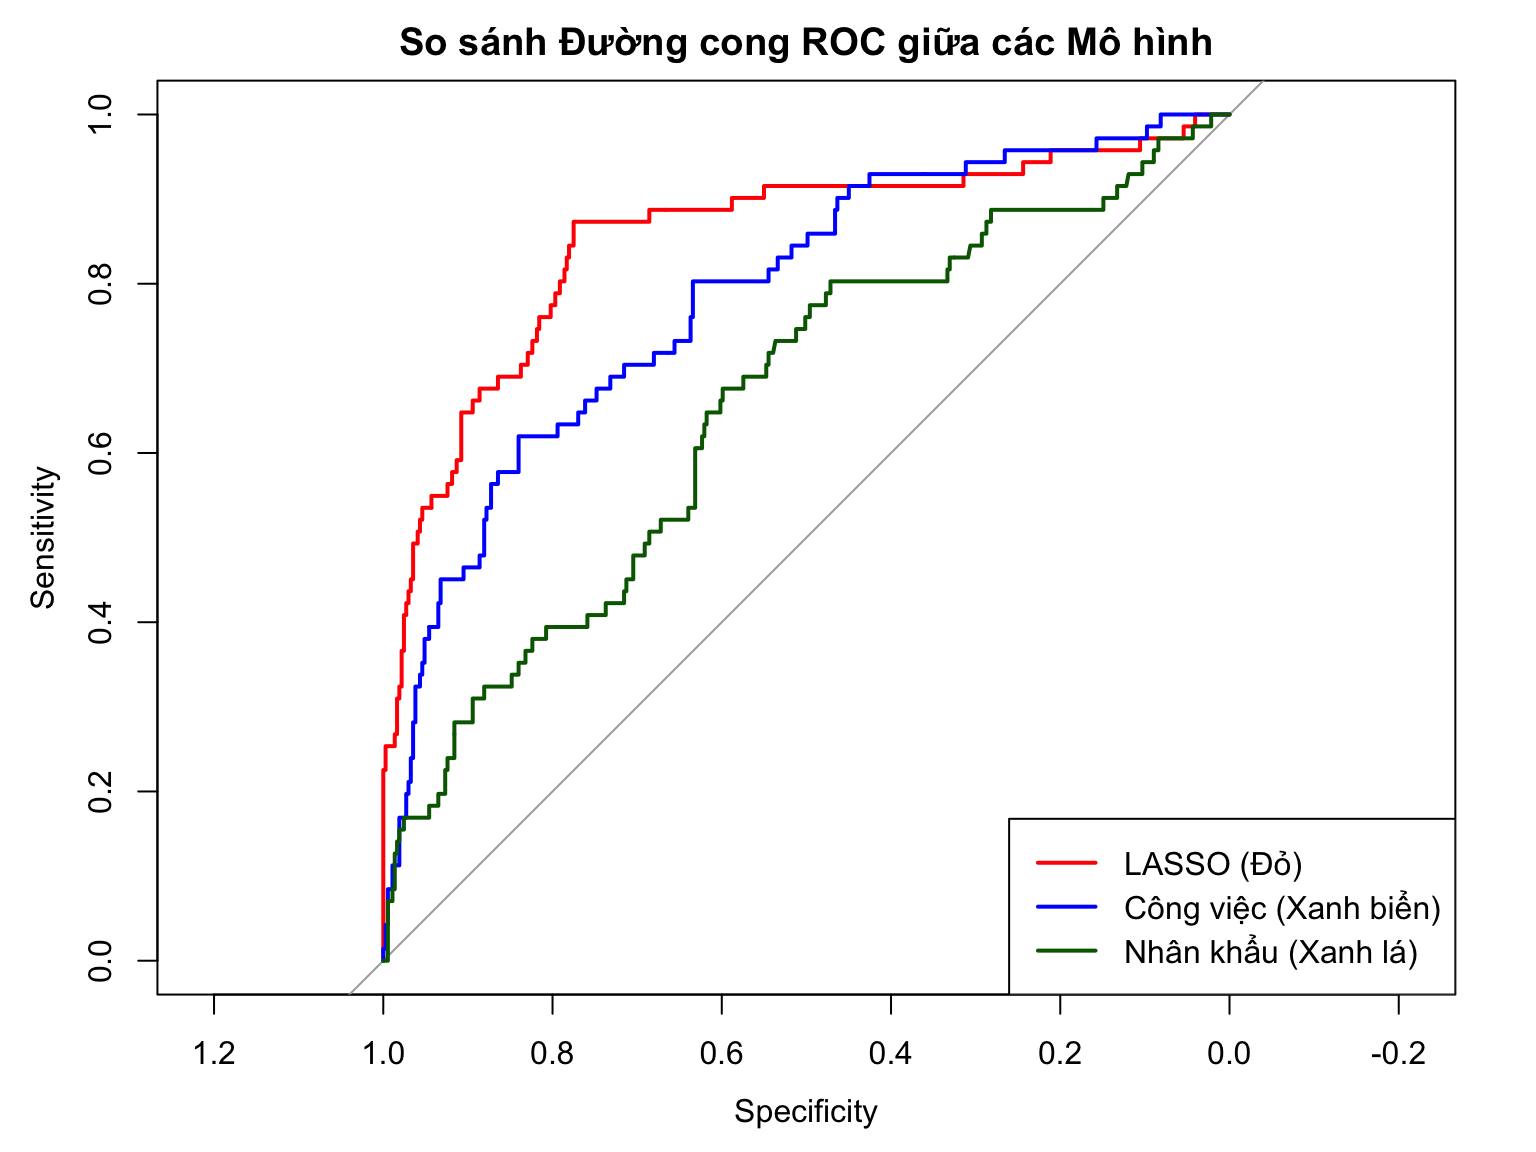
\includegraphics[width=\linewidth,height=5.20cm,keepaspectratio,
        trim=35 35 22 25,clip]{img/hr-roc-logistic-models.png}
    \end{column}
  \end{columns}
\end{frame}

% Thời lượng: 1:15
% Thông điệp: Ngưỡng 0,5 mặc định không hợp với lớp thiểu số 16%;
% quét dãy ngưỡng và chọn 0,30 theo tiêu chí cực đại F1.
\begin{frame}{Chọn ngưỡng quyết định 0,30 bằng tiêu chí F1}
  \begin{columns}[T,onlytextwidth]
    \begin{column}{0.65\textwidth}
      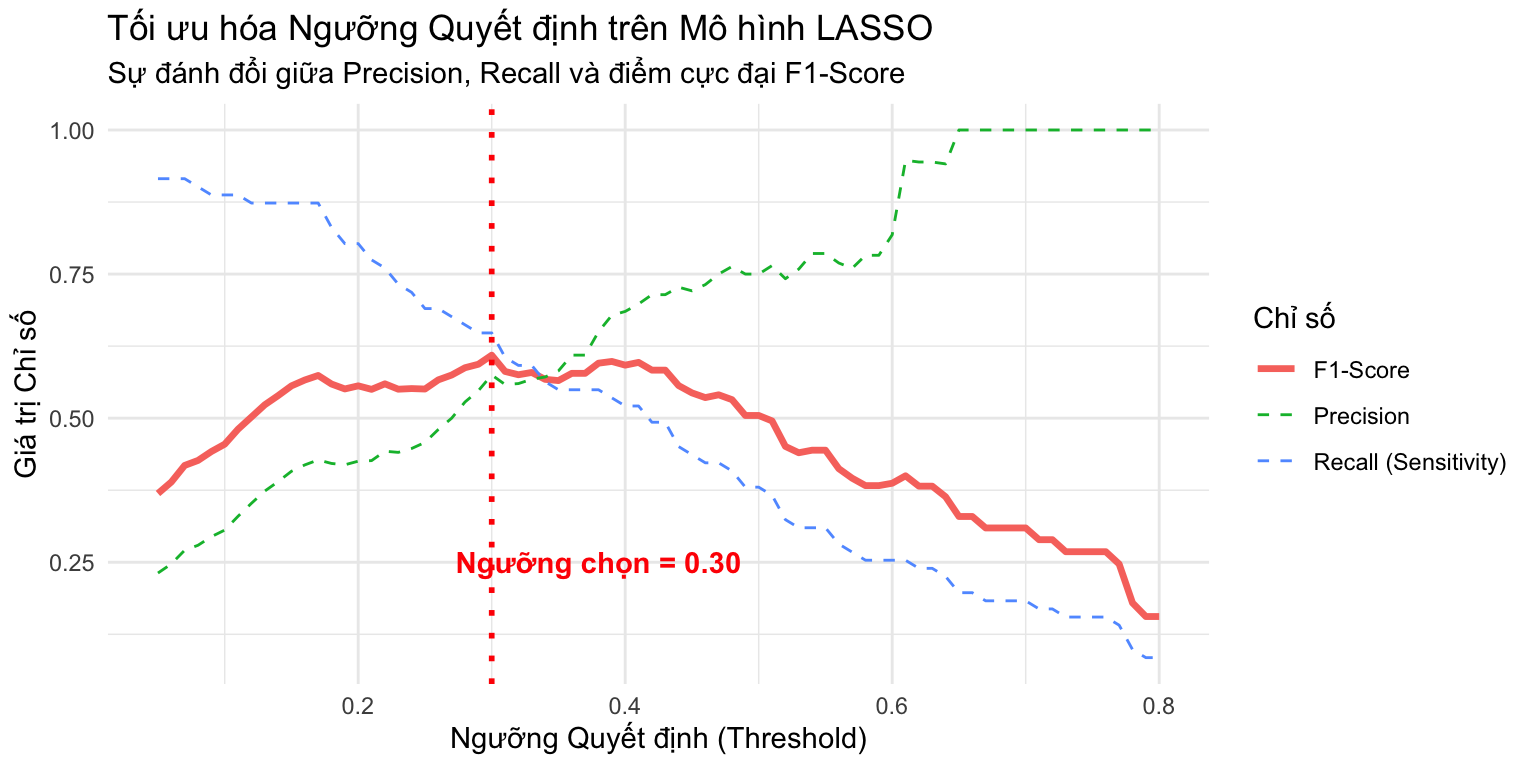
\includegraphics[width=\linewidth,height=5.55cm,keepaspectratio,
        trim=20 18 120 20,clip]{img/hr-threshold-optimization.png}
    \end{column}
    \begin{column}{0.32\textwidth}
      \begin{beamercolorbox}[sep=0.18cm,rounded=true]{block body}
        \centering
        \textbf{\color{HCMUSRed}\Large 0,30}\\
        \small Cực đại F1 $=0{,}609$\\
        Sensitivity: \textbf{64,8\%}\\
        Specificity: \textbf{90,8\%}
      \end{beamercolorbox}
      \vspace{0.20cm}
      \begin{beamercolorbox}[sep=0.18cm,rounded=true]{block body}
        \small
        \textbf{Vì sao không dùng 0,5?}\\[0.04cm]
        Lớp nghỉ việc chỉ chiếm 16\%: ngưỡng mặc định bỏ sót phần lớn
        ca rủi ro. Hạ ngưỡng giúp tăng khả năng phát hiện.
      \end{beamercolorbox}
      \vspace{0.20cm}
      {\scriptsize\color{MutedText}
       Tiêu chí thay thế (Youden, hàm chi phí) cho ngưỡng thấp hơn,
       $\approx 0{,}17$ --- chi tiết ở phụ lục B3.}
    \end{column}
  \end{columns}
\end{frame}

% Thời lượng: 0:45
% Thông điệp: Tập trung vào yếu tố can thiệp được và luôn có con người rà soát.
\begin{frame}{Từ mô hình đến hành động HR}
  \begin{columns}[T,onlytextwidth]
    \begin{column}{0.48\textwidth}
      \begin{block}{1. Kiểm soát làm thêm giờ}
        \small Theo dõi OT theo nhóm, phân bổ lại tải việc và đo lường
        kiệt sức định kỳ.
      \end{block}
      \vspace{0.12cm}
      \begin{block}{2. Can thiệp theo chức danh}
        \small Stay interview và khảo sát ẩn danh cho các vai trò có
        tín hiệu rủi ro cao.
      \end{block}
    \end{column}
    \begin{column}{0.48\textwidth}
      \begin{block}{3. Cải thiện trải nghiệm}
        \small Theo dõi hài lòng, lộ trình nghề nghiệp, đào tạo và cơ hội
        luân chuyển nội bộ.
      \end{block}
      \vspace{0.12cm}
      \begin{block}{4. Cảnh báo sớm có giám sát}
        \small Chấm điểm định kỳ, hiệu chỉnh ngưỡng bằng chi phí thực tế
        và luôn yêu cầu HR rà soát.
      \end{block}
    \end{column}
  \end{columns}
  \vspace{0.15cm}
  \begin{beamercolorbox}[sep=0.15cm,rounded=true]{alerted text}
    \centering\small
    \textbf{Không dùng điểm rủi ro để kỷ luật hoặc sa thải tự động.}
    Kiểm tra fairness, quyền riêng tư và cơ sở pháp lý trước khi triển khai.
  \end{beamercolorbox}
\end{frame}

% Thời lượng: 0:45
% Thông điệp: Kết quả minh họa quy trình tốt nhưng chưa đủ điều kiện triển khai.
\begin{frame}{Giới hạn cần xử lý trước khi triển khai}
  \begin{columns}[T,onlytextwidth]
    \begin{column}{0.48\textwidth}
      \begin{beamercolorbox}[sep=0.18cm,rounded=true]{block body}
        \textbf{Tính đại diện}\\
        \small Dữ liệu mô phỏng, lát cắt và không có thời gian đến khi
        nghỉ việc; chưa thể khái quát cho doanh nghiệp cụ thể.
      \end{beamercolorbox}
      \vspace{0.18cm}
      \begin{beamercolorbox}[sep=0.18cm,rounded=true]{block body}
        \textbf{Đánh giá hiệu suất}\\
        \small Ngưỡng đang được khảo sát trên test; cần chọn trong
        validation hoặc nested cross-validation.
      \end{beamercolorbox}
    \end{column}
    \begin{column}{0.48\textwidth}
      \begin{beamercolorbox}[sep=0.18cm,rounded=true]{block body}
        \textbf{Độ tin cậy xác suất}\\
        \small Bổ sung PR-AUC, Brier score, calibration curve và khoảng
        tin cậy bootstrap cho AUC.
      \end{beamercolorbox}
      \vspace{0.18cm}
      \begin{beamercolorbox}[sep=0.18cm,rounded=true]{block body}
        \textbf{Quản trị mô hình}\\
        \small Kiểm định trên dữ liệu thật, theo dõi drift, fairness và
        hiệu chỉnh ngưỡng theo chi phí vận hành.
      \end{beamercolorbox}
    \end{column}
  \end{columns}
\end{frame}

% Thời lượng: 0:45
% Thông điệp: Chốt đúng ba ý; dừng ở đây để dành thời gian cho câu hỏi.
\begin{frame}{Ba kết luận chính}
  \vspace{0.18cm}
  \begin{enumerate}
    \item \textbf{Điều kiện công việc quan trọng hơn nhân khẩu học:}\\
          làm thêm giờ, sự hài lòng và chức danh tạo tín hiệu dự báo rõ nhất.
    \vspace{0.28cm}
    \item \textbf{LASSO là lựa chọn cân bằng nhất:}\\
          AUC \(=0,854\), sensitivity \(=64,8\%\), F1 \(=0,609\) tại
          ngưỡng 0,30.
    \vspace{0.28cm}
    \item \textbf{Mô hình là công cụ hỗ trợ can thiệp:}\\
          ưu tiên cải thiện tải việc và trải nghiệm nhân viên, không tự
          động gắn nhãn hay ra quyết định bất lợi.
  \end{enumerate}

  \vfill
  \begin{beamercolorbox}[sep=0.18cm,center,rounded=true]{block body}
    {\Large\bfseries\color{HCMUSBlue}Cảm ơn Thầy/Cô và các bạn!}
    \qquad {\large Câu hỏi \& thảo luận}
  \end{beamercolorbox}
\end{frame}

% ==================== BACKUP / Q&A ====================
% Các slide sau không nằm trong mạch trình bày 15 phút;
% chỉ bật ra khi được hỏi trong phần thảo luận.
\appendix

\begin{frame}[plain]
  \vfill\centering
  {\Large\bfseries\color{HCMUSBlue} Backup --- Hỏi \& đáp}\\[0.25cm]
  {\small\color{MutedText} Các slide sau chỉ dùng khi thảo luận.}
  \vfill
\end{frame}

% B1: khi được hỏi về kiểm tra đa cộng tuyến / giả định logistic.
\begin{frame}{B1. Kiểm tra đa cộng tuyến: VIF/GVIF chi tiết}
  \begin{columns}[T,onlytextwidth]
    \begin{column}{0.48\textwidth}
      \centering\small
      \textbf{Mô hình nhân khẩu học}\\[0.12cm]
      \scriptsize
      \renewcommand{\arraystretch}{1.2}
      \begin{tabular}{lrr}
        \toprule
        Biến & VIF & GVIF\\
        \midrule
        Age\_scaled & 1,101 & 1,101\\
        Gender & 1,011 & 1,011\\
        MaritalStatus & --- & 1,023\\
        DistanceFromHome & 1,008 & 1,008\\
        Education & 1,090 & 1,090\\
        \bottomrule
      \end{tabular}
    \end{column}
    \begin{column}{0.48\textwidth}
      \centering\small
      \textbf{Mô hình công việc (đã loại Department)}\\[0.12cm]
      \scriptsize
      \renewcommand{\arraystretch}{1.2}
      \begin{tabular}{lrr}
        \toprule
        Biến & VIF & GVIF\\
        \midrule
        JobRole & --- & 2,935\\
        EnvironmentSatisfaction & 1,042 & 1,042\\
        JobSatisfaction & 1,013 & 1,013\\
        OverTime & 1,090 & 1,090\\
        Income\_scaled & 2,816 & 2,816\\
        \bottomrule
      \end{tabular}
    \end{column}
  \end{columns}
  \vspace{0.28cm}
  \begin{beamercolorbox}[sep=0.14cm,rounded=true]{block body}
    \small
    Tất cả dưới ngưỡng tham khảo 5. Lưu ý: VIF thấp cho biết không có
    cộng tuyến tuyến tính mạnh giữa các biến giải thích, nhưng không đồng
    nghĩa chúng độc lập thống kê hoàn toàn.
  \end{beamercolorbox}
\end{frame}

% B2: khi được hỏi vì sao không dùng hẳn ML, hoặc RF/GBM thế nào.
\begin{frame}{B2. Mô hình phi tuyến: Random Forest và GBM}
  \begin{columns}[T,onlytextwidth]
    \begin{column}{0.52\textwidth}
      \centering\scriptsize
      \renewcommand{\arraystretch}{1.25}
      \begin{tabular}{lccccc}
        \toprule
        & \textbf{AUC} & \textbf{Acc.} & \textbf{Sens.} & \textbf{Prec.} & \textbf{F1}\\
        \midrule
        \rowcolor{HCMUSLight}
        \textbf{LASSO} & \textbf{0,854} & \textbf{0,866} & \textbf{0,648} & 0,575 & \textbf{0,609}\\
        RF (classwt 1:5) & 0,796 & 0,827 & 0,479 & 0,466 & 0,472\\
        GBM & 0,841 & 0,859 & 0,465 & \textbf{0,579} & 0,516\\
        \bottomrule
      \end{tabular}
      \vspace{0.18cm}

      \small
      RF: 300 cây, nodesize 5, trọng số lớp 1:5.\\
      GBM: 150 cây, depth 3, shrinkage 0,05, 5-fold CV.
      % \vspace{0.18cm}
      % \begin{beamercolorbox}[sep=0.13cm,rounded=true]{block body}
      %   \small \textbf{Chiến lược phối hợp:} LASSO recall cao để quét rộng;
      %   GBM precision cao để ưu tiên ngân sách giữ chân có hạn.
      %   Không kết luận RF ``overfit'' khi chưa so sánh train/CV.
      % \end{beamercolorbox}
    \end{column}
    \begin{column}{0.46\textwidth}
      \centering
      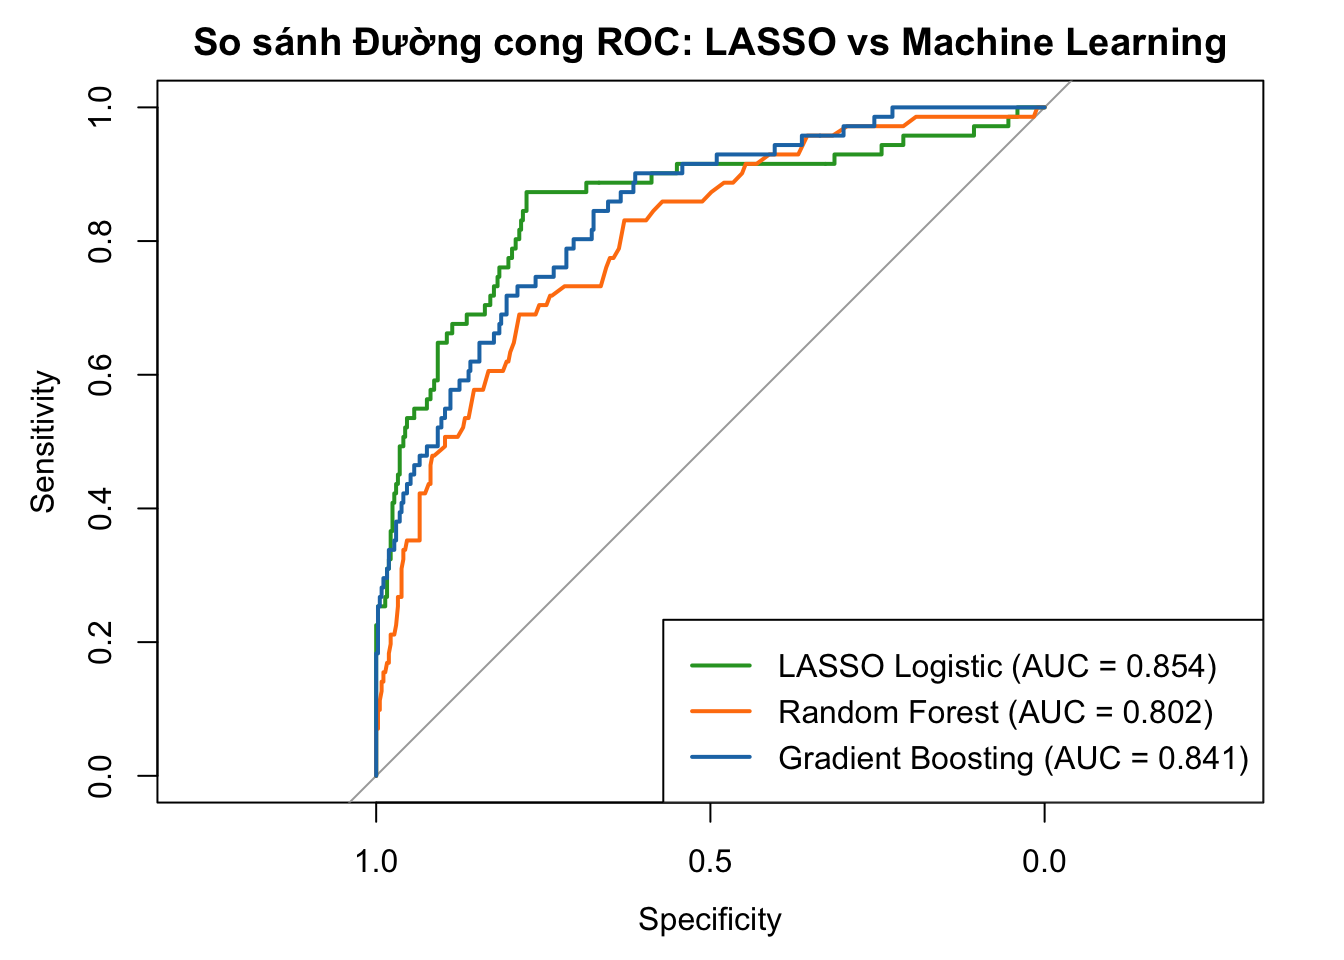
\includegraphics[width=\linewidth,height=5.5cm,keepaspectratio]
        {img/hr-roc-advanced-models.png}\\[-0.05cm]
      {\tiny\color{MutedText}
       Lưu ý: chú giải ROC trong HTML ghi cứng RF AUC \(=0,802\);
       bảng kết quả tính trực tiếp cho \(0,796\), được dùng trong slide.}
    \end{column}
  \end{columns}
\end{frame}

% B3: khi được hỏi vì sao ngưỡng 0,30 / chi phí lấy đâu ra.
\begin{frame}{B3. Ba tiêu chí chọn ngưỡng quyết định}
  \begin{columns}[T,onlytextwidth]
    \begin{column}{0.55\textwidth}
      \small
      Quét ngưỡng $0{,}05 \to 0{,}80$ (bước $0{,}01$) trên xác suất LASSO
      của tập test:
      \vspace{0.15cm}
      \begin{enumerate}
        \item \textbf{Tối đa F1} $\Rightarrow$ ngưỡng \textbf{0,30}
              (F1 $= 0{,}609$)
        \item \textbf{Youden's J} (Sens + Spec $-$ 1) $\Rightarrow$
              ngưỡng \textbf{0,17}
        \item \textbf{Tối thiểu chi phí} với giả định
              FN $= 15.000$ USD, FP $= 1.000$ USD $\Rightarrow$
              ngưỡng \textbf{0,17}
      \end{enumerate}
    \end{column}
    \begin{column}{0.42\textwidth}
      \begin{beamercolorbox}[sep=0.16cm,rounded=true]{block body}
        \small
        \textbf{Kết luận:} không có ngưỡng tối ưu duy nhất cho mọi mục tiêu
        --- lựa chọn phụ thuộc chi phí sai sót của tổ chức.
      \end{beamercolorbox}
      \vspace{0.16cm}
      \begin{beamercolorbox}[sep=0.16cm,rounded=true]{alerted text}
        \small
        Chi phí FN/FP là giả định minh họa (tham khảo chi phí thay thế
        nhân sự); khi triển khai cần hiệu chỉnh bằng chi phí thực và chọn
        ngưỡng trên tập validation, không phải test.
      \end{beamercolorbox}
    \end{column}
  \end{columns}
\end{frame}

% B4: khi được hỏi vì sao không SMOTE / độ tin cậy của một lần chia.
\begin{frame}{B4. Mất cân bằng lớp và độ tin cậy ước lượng}
  \begin{columns}[T,onlytextwidth]
    \begin{column}{0.48\textwidth}
      \begin{block}{Đã xử lý bằng gì?}
        \small
        Chia phân tầng giữ tỷ lệ 16,12\% ở cả hai tập; hạ ngưỡng về 0,30;
        đánh giá bằng AUC, sensitivity, F1 thay cho accuracy;
        trọng số lớp 1:5 trong Random Forest.
      \end{block}
      \vspace{0.14cm}
      \begin{block}{Vì sao chưa SMOTE/ROSE?}
        \small
        Giữ phân phối gốc để xác suất dự báo phản ánh tỷ lệ thật;
        mẫu tổng hợp có rủi ro thêm nhiễu. Đây là hướng cải thiện
        đã nêu trong báo cáo, không phải thiếu sót bị bỏ qua.
      \end{block}
    \end{column}
    \begin{column}{0.48\textwidth}
      \begin{block}{Giới hạn thừa nhận}
        \small
        Kết quả dựa trên một lần chia 70/30 (seed 123) --- các chỉ số là
        ước lượng điểm. Khoảng tin cậy 95\% cho accuracy LASSO:
        $[0{,}830;\ 0{,}896]$.
      \end{block}
      \vspace{0.14cm}
      \begin{beamercolorbox}[sep=0.15cm,rounded=true]{block body}
        \small
        \textbf{Hướng nâng cấp:} repeated k-fold CV cho toàn pipeline,
        bootstrap CI cho AUC, và so sánh có kiểm định (DeLong) giữa các
        mô hình.
      \end{beamercolorbox}
    \end{column}
  \end{columns}
\end{frame}

% B5: khi được hỏi con số phân loại cụ thể trên test.
\begin{frame}{B5. Ma trận nhầm lẫn LASSO trên test (ngưỡng 0,30)}
  \begin{columns}[T,onlytextwidth]
    \begin{column}{0.44\textwidth}
      \centering\small
      \renewcommand{\arraystretch}{1.4}
      \begin{tabular}{l|cc}
        & \textbf{Thực: No} & \textbf{Thực: Yes}\\
        \hline
        \textbf{Dự báo No} & \cellcolor{HCMUSLight}335 (TN) & 25 (FN)\\
        \textbf{Dự báo Yes} & 34 (FP) & \cellcolor{HCMUSLight}46 (TP)\\
      \end{tabular}
      \vspace{0.2cm}

      \small Tập test $n = 440$ (369 No / 71 Yes)
    \end{column}
    \begin{column}{0.52\textwidth}
      \small
      \begin{itemize}
        \item Sensitivity (recall): $46/71 = \textbf{64,8\%}$
        \item Specificity: $335/369 = \textbf{90,8\%}$
        \item Precision: $46/80 = \textbf{57,5\%}$; F1 $= \textbf{0,609}$
        \item Accuracy: $\textbf{86,6\%}$, CI 95\% $[0{,}830;\ 0{,}896]$;
              Kappa $= 0{,}529$
        \item Balanced accuracy: $77{,}8\%$
      \end{itemize}
      \vspace{0.10cm}
      \begin{beamercolorbox}[sep=0.13cm,rounded=true]{block body}
        \small Bỏ sót 25/71 ca nghỉ việc --- lý do cân nhắc ngưỡng 0,17
        cho tầng theo dõi rộng (chấp nhận thêm false positive).
      \end{beamercolorbox}
    \end{column}
  \end{columns}
\end{frame}

% B6: khi được hỏi về các lựa chọn phương pháp luận.
\begin{frame}{B6. Vì sao chọn các phương pháp này?}
  \small
  \begin{itemize}
    \item \textbf{Logistic làm trục chính, không phải ML thuần:}
          hệ số $\to$ odds ratio diễn giải được cho HR; và thực nghiệm
          cho thấy LASSO thắng cả RF/GBM về AUC trên bộ dữ liệu này.
    \vspace{0.12cm}
    \item \textbf{$\lambda_{\min}$ thay vì $\lambda_{1se}$:}
          mục tiêu chính là năng lực dự báo; $\lambda_{1se}$ (29 biến)
          được báo cáo làm đối chứng cho phương án triển khai gọn.
    \vspace{0.12cm}
    \item \textbf{Không dùng stepwise:} chọn biến từng bước không ổn định
          và làm sai lệch suy luận sau chọn biến; phạt L1 của LASSO là
          cách chọn biến có kiểm soát chính quy hóa, chọn bằng CV.
    \vspace{0.12cm}
    \item \textbf{Chia 70/30 phân tầng, seed cố định:} giữ nguyên tỷ lệ
          lớp hiếm ở hai tập và bảo đảm tái lập được toàn bộ kết quả.
    \vspace{0.12cm}
    \item \textbf{Kiểm định phi tham số (Wilcoxon):} Shapiro--Wilk bác bỏ
          tính chuẩn của thu nhập trong nhóm nghỉ việc nên không dùng t-test.
  \end{itemize}
\end{frame}

% B7: khi được hỏi "LASSO giữ biến nào?". Hệ số tái lập từ pipeline seed 123
% (báo cáo chỉ nêu tổng số 35); hệ số trên thang biến đã chuẩn hóa/dummy.
\begin{frame}{B7. LASSO giữ biến nào tại $\lambda_{\min}$?}
  \begin{columns}[T,onlytextwidth]
    \begin{column}{0.48\textwidth}
      \centering\small
      \textbf{\color{HCMUSRed}Hệ số dương lớn nhất (tăng nguy cơ)}\\[0.10cm]
      \scriptsize
      \renewcommand{\arraystretch}{1.2}
      \begin{tabular}{lr}
        \toprule
        BusinessTravel: Frequently & $+1{,}77$\\
        OverTime: Yes & $+1{,}67$\\
        JobRole: Sales Representative & $+1{,}08$\\
        MaritalStatus: Single & $+0{,}95$\\
        JobRole: Laboratory Technician & $+0{,}94$\\
        JobRole: Human Resources & $+0{,}92$\\
        \bottomrule
      \end{tabular}
    \end{column}
    \begin{column}{0.48\textwidth}
      \centering\small
      \textbf{\color{HCMUSGreen}Hệ số âm lớn nhất (giảm nguy cơ)}\\[0.10cm]
      \scriptsize
      \renewcommand{\arraystretch}{1.2}
      \begin{tabular}{lr}
        \toprule
        JobRole: Research Director & $-0{,}93$\\
        JobInvolvement & $-0{,}39$\\
        EnvironmentSatisfaction & $-0{,}38$\\
        JobSatisfaction & $-0{,}34$\\
        JobRole: Manager & $-0{,}31$\\
        WorkLifeBalance & $-0{,}27$\\
        \bottomrule
      \end{tabular}
    \end{column}
  \end{columns}
  \vspace{0.25cm}
  \begin{beamercolorbox}[sep=0.14cm,rounded=true]{block body}
    \small
    Tổng cộng 35 hệ số $\neq 0$. Thu nhập bị co về đúng 0 --- nhất quán với
    $p = 0{,}968$ ở mô hình công việc. Hệ số trên thang biến chuẩn hóa/dummy,
    tái lập từ pipeline với seed 123.
  \end{beamercolorbox}
\end{frame}

% B8: khi được hỏi về AIC hoặc các giả định của hồi quy Logistic.
\begin{frame}{B8. AIC và các giả định cần kiểm tra}
  \begin{columns}[T,onlytextwidth]
    \begin{column}{0.43\textwidth}
      \begin{block}{Cách đọc AIC}
        \small
        \[
          AIC=-2\log(\widehat L)+2k
        \]
        AIC cân bằng độ phù hợp và độ phức tạp; \textbf{càng thấp càng
        tốt} khi so sánh mô hình dùng cùng dữ liệu và biến phản hồi.
      \end{block}
      \vspace{0.12cm}
      \begin{beamercolorbox}[sep=0.14cm,rounded=true]{block body}
        \small
        Mô hình công việc: \(781,32\), thấp hơn mô hình nhân khẩu học
        \(858,89\). LASSO không dùng AIC truyền thống trong phân tích này
        vì hàm mục tiêu chứa hình phạt \(L_1\); \(\lambda\) được chọn bằng
        cross-validation.
      \end{beamercolorbox}
    \end{column}
    \begin{column}{0.54\textwidth}
      \begin{block}{Đã đáp ứng hoặc đã kiểm tra}
        \small
        \begin{itemize}
          \item Phản hồi nhị phân \texttt{Yes}/\texttt{No}.
          \item Không có đa cộng tuyến nghiêm trọng sau khi bỏ
                \texttt{Department}; GVIF hiệu chỉnh \(<5\).
          \item Mô hình hội tụ và không còn dấu hiệu hệ số suy biến.
        \end{itemize}
      \end{block}
      \vspace{0.10cm}
      \begin{block}{Chưa thể khẳng định hoàn toàn}
        \small
        \begin{itemize}
          \item Độc lập quan sát nếu nhân viên cùng nhóm/quản lý.
          \item Tuyến tính giữa biến liên tục và log-odds
                (cần spline, GAM hoặc Box--Tidwell).
          \item Calibration của xác suất (cần Brier score và
                calibration curve).
        \end{itemize}
      \end{block}
    \end{column}
  \end{columns}
\end{frame}

\end{document}
